\section{Experimental Evaluation}\label{sec:experiments}
In this section, we present a comprehensive experimental evaluation 
of our solutions using several real-world information networks and 
various synthetic datasets. Since the focus of this paper is on query processing efficiency, 
we do not evaluate the efficiency of index updates. 
All experiments are conducted on an 
Amazon EC2 r3.2xlarge machine\footnote{http://aws.amazon.com/ec2/pricing/}, 
with an 8-core 2.5GHz CPU, 60GB memory and 320GB hard drive 
running with 64-bit Ubuntu 12.04. As the source code of EAGR is not
available, we implemented it and used it as a reference in our comparative
study.  
All algorithms are implemented in Java and run under JRE 1.6.

\begin{table}[h]
\centering
\begin{tabular}{|l|l|l|l|}
\hline 
\rule[-1ex]{0pt}{2.5ex} Name & Type & \# of Vertices & \# of Edges \\ 
\hline 
\rule[-1ex]{0pt}{2.5ex} LiveJournal1 & undirected & 3,997,962 & 34,681,189 \\ 
\hline 
\rule[-1ex]{0pt}{2.5ex} Pokec & directed & 1,632,803 & 30,622,564 \\ 
\hline 
\rule[-1ex]{0pt}{2.5ex} Orkut & undirected & 3,072,441 & 117,185,083 \\ 
\hline 
\rule[-1ex]{0pt}{2.5ex} DBLP & undirected & 317,080 & 1,049,866 \\ 
\hline 
\rule[-1ex]{0pt}{2.5ex} YouTube & undirected & 1,134,890 & 2,987,624 \\ 
\hline 
\rule[-1ex]{0pt}{2.5ex} Google & directed & 875,713 & 5,105,039 \\ 
\hline 
\rule[-1ex]{0pt}{2.5ex} Amazon & undirected & 334,863 & 925,872 \\ 
\hline 
\rule[-1ex]{0pt}{2.5ex} Stanford-web & directed & 281,903 &  2,312,497 \\ 
\hline 
\end{tabular}
\caption{Large Scale Real Data}
\label{tab:realdata}
\end{table}


\textbf{Datasets.} For real datasets, we use 8 information networks 
which are available at the Stanford \emph{SNAP} 
website \footnote{http://snap.stanford.edu/snap/index.html}: 
LiveJournal1, Pokec, Orkut, DBLP, YouTube, Google, Amazon and Stanford-web. 
The detail description of these datasets is provided in 
Table~\ref{tab:realdata}. 

For synthetic datasets, we use two widely used graph data generators. 
We use the \emph{DAGGER} generator \cite{yildirim2013dagger} to generate 
all the synthetic DAGs and the SNAP graph data generator at the
Stanford SNAP website to generate non-DAG datasets. For each dataset, each vertex is associated with an integer attribute.

\textbf{Query.} In all the experiments, the window query is conducted 
by using the SUM() as the aggregate function over the integer attribute in each dataset. 

\begin{figure*}[t]
\centering
\begin{subfigure}{0.23\textwidth}
  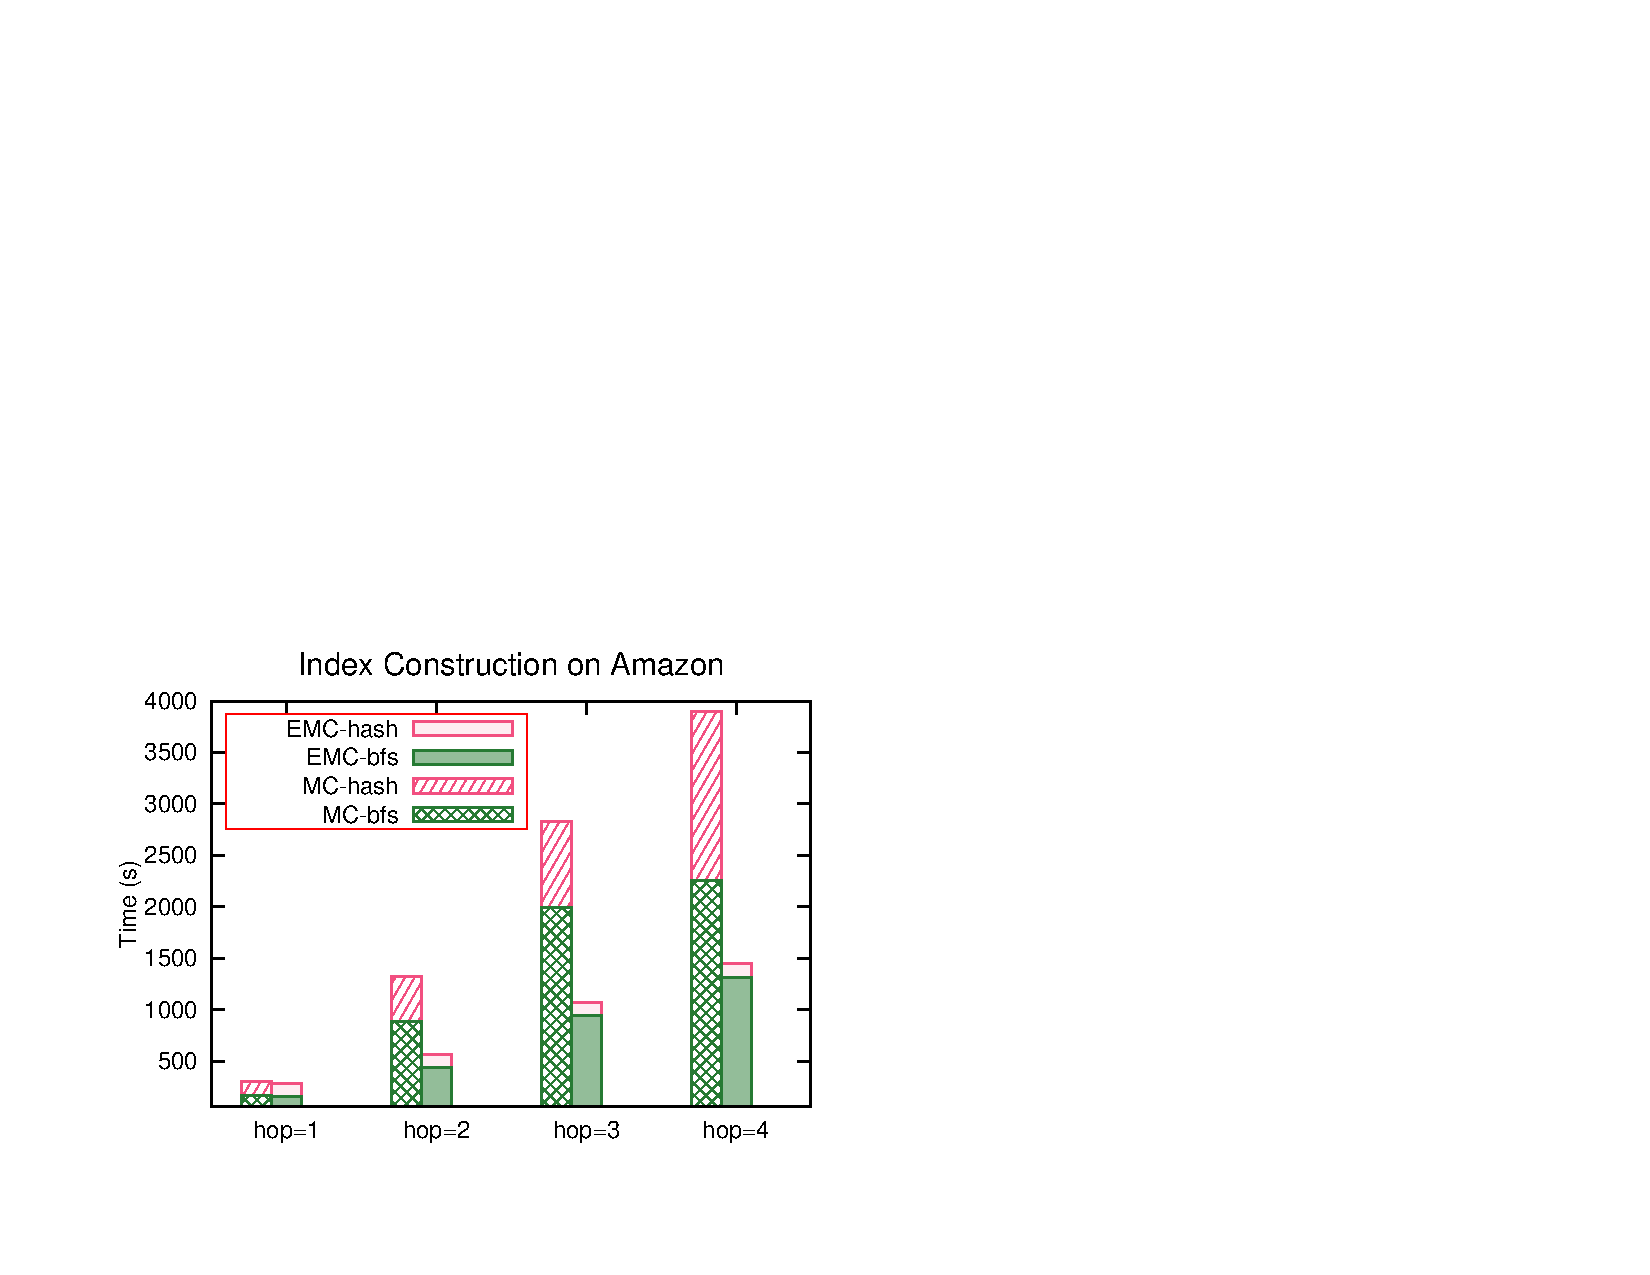
\includegraphics[width=\textwidth]{chapter3/exp/khopeffect/effectiveness/amazon_index_time.pdf}
  \caption{Index Built on Amazon}
\end{subfigure}
\begin{subfigure}{0.23\textwidth}
  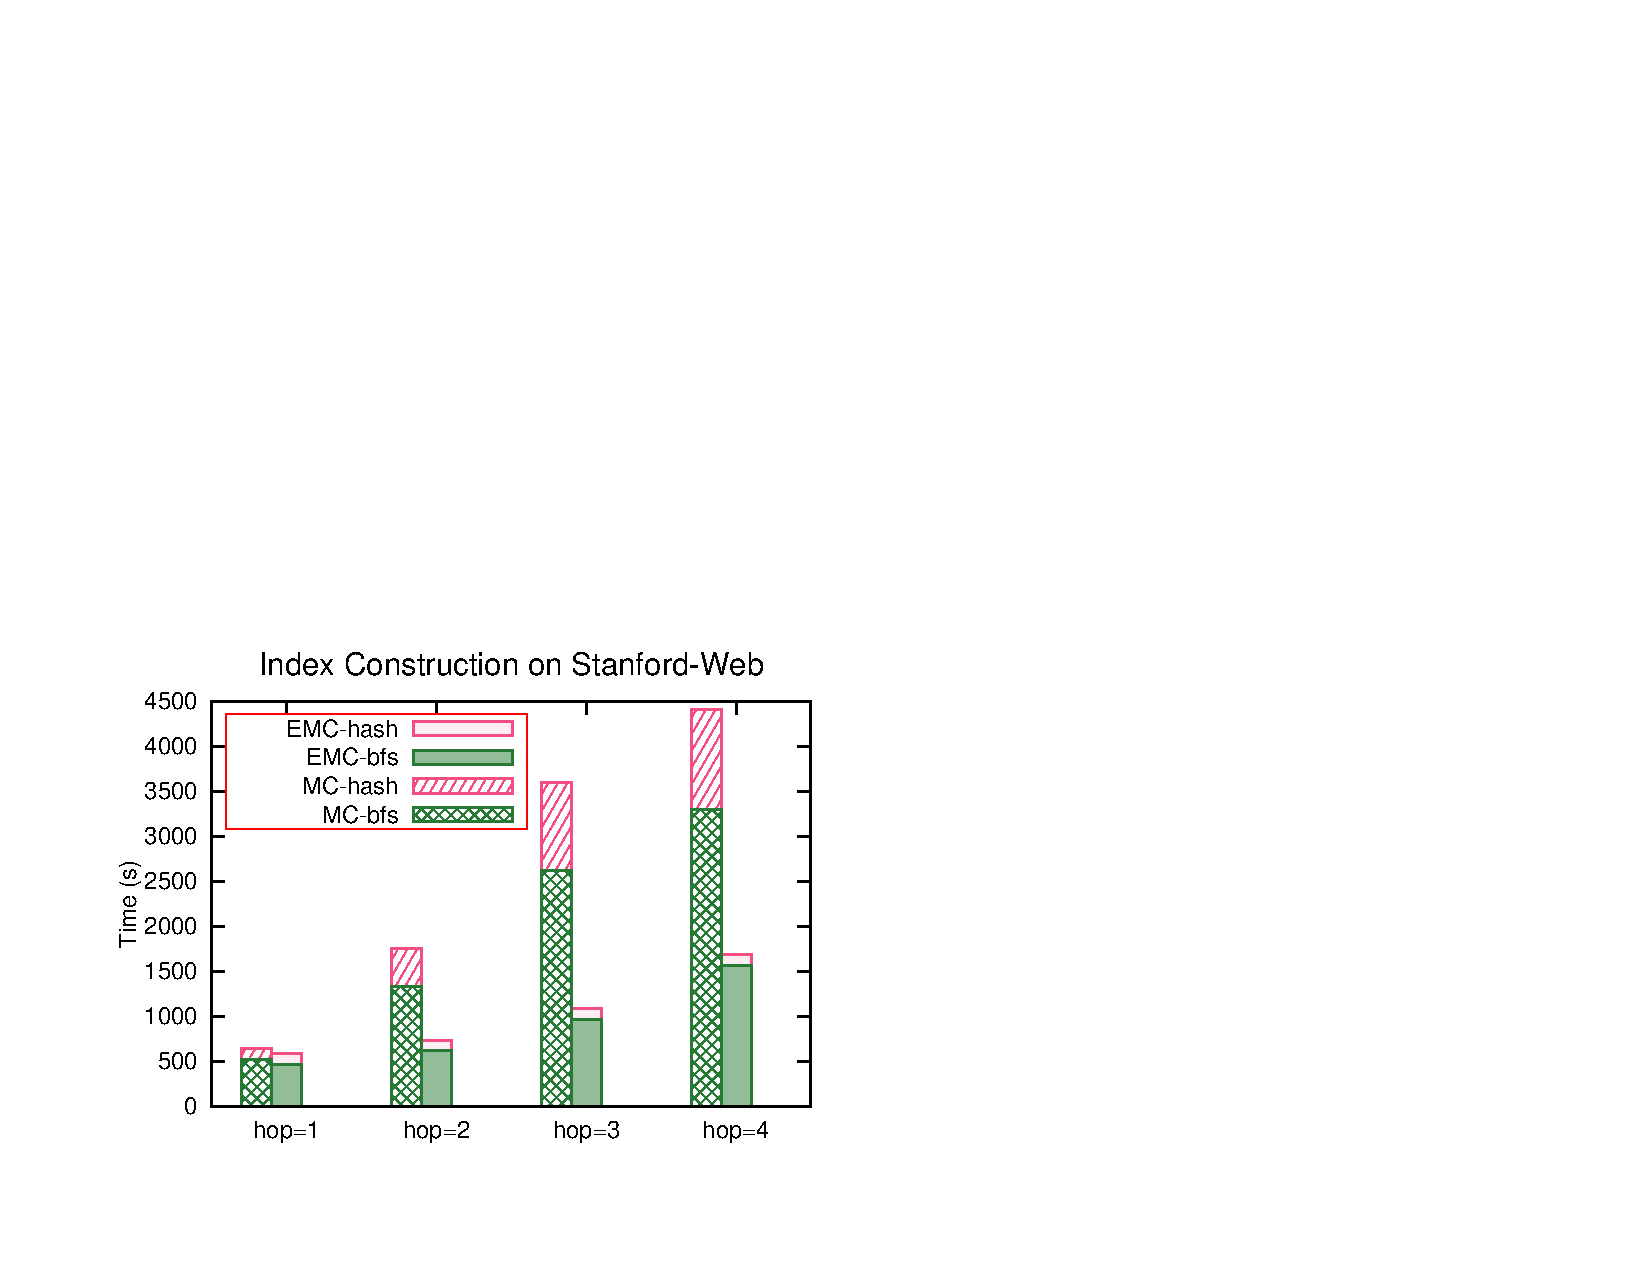
\includegraphics[width=\textwidth]{chapter3/exp/khopeffect/effectiveness/stanford_index_time.pdf}
  \caption{Index Built on Stanford-web}
\end{subfigure}
\begin{subfigure}{0.23\textwidth}
  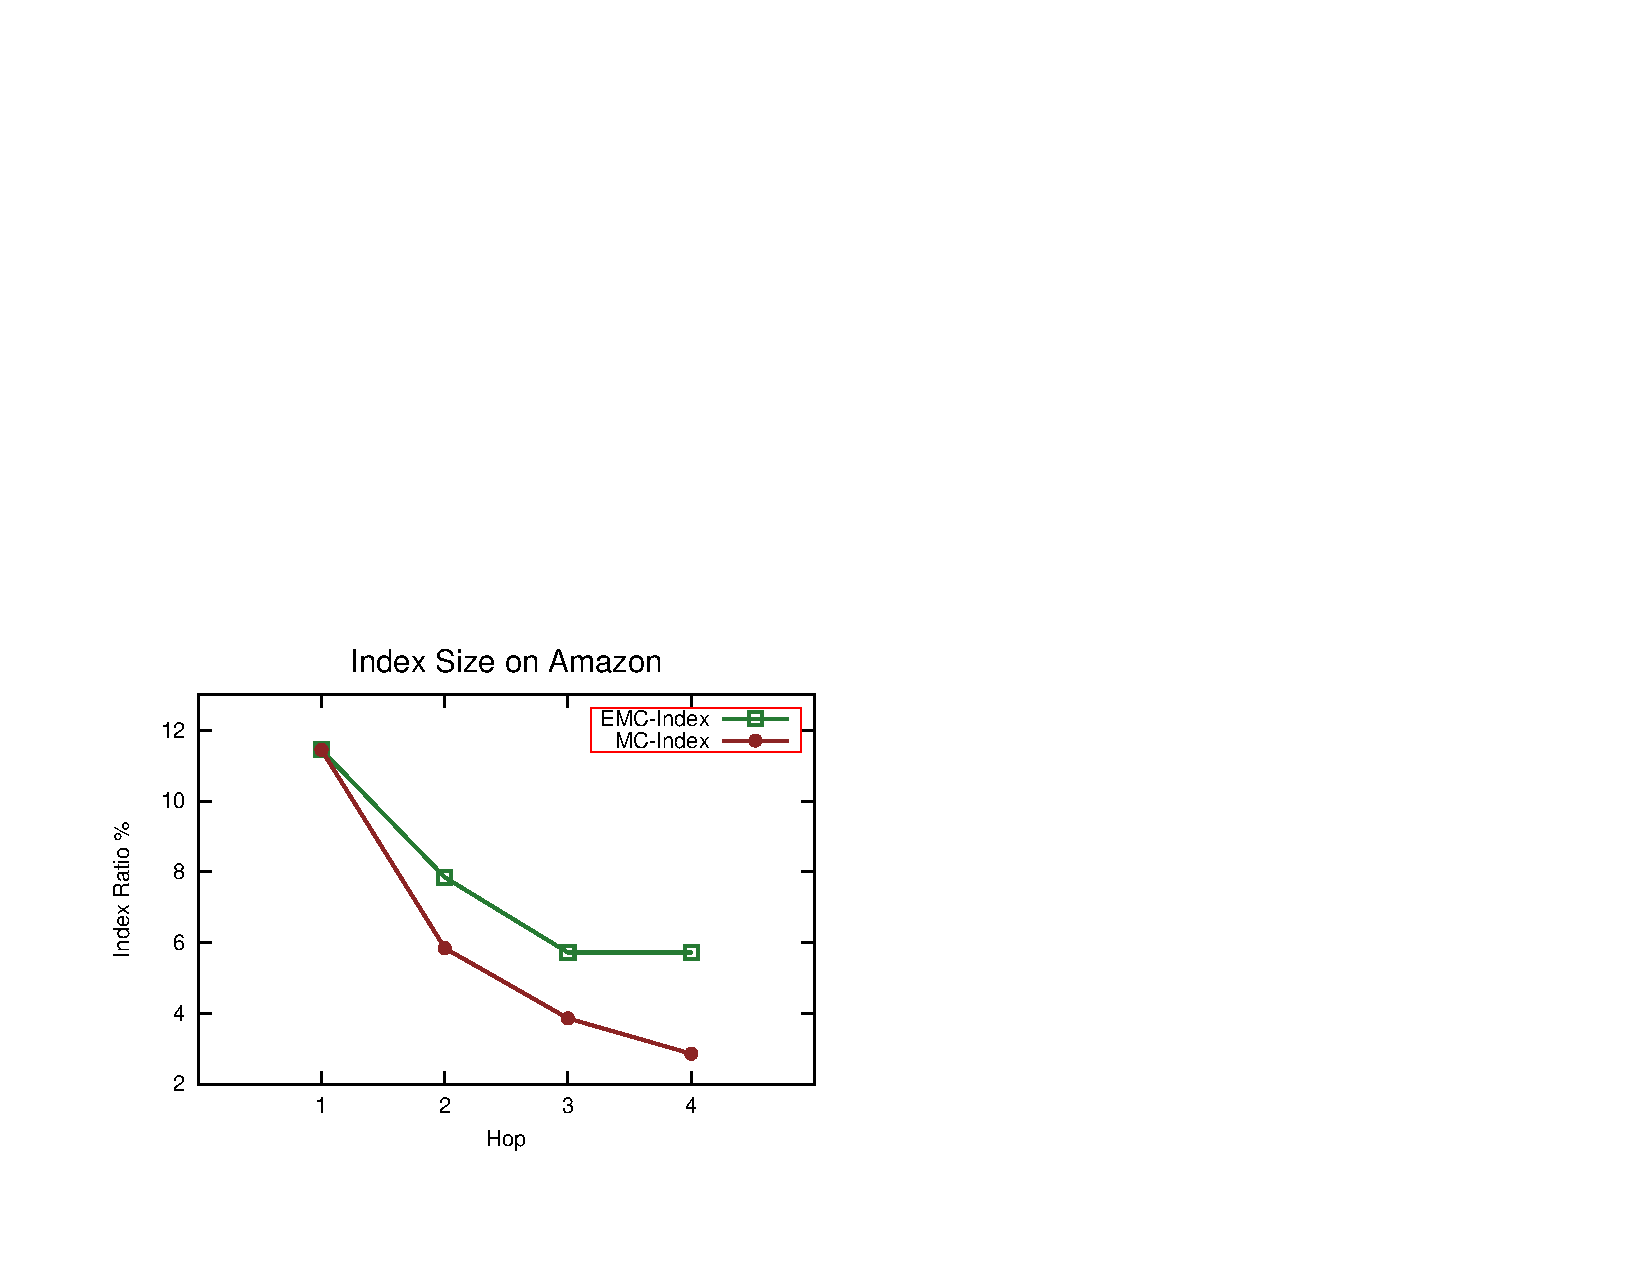
\includegraphics[width=\textwidth]{chapter3/exp/khopeffect/effectiveness/amazon_index_size.pdf}
  \caption{Index Size on Amazon}
\end{subfigure}
\begin{subfigure}{0.23\textwidth}
  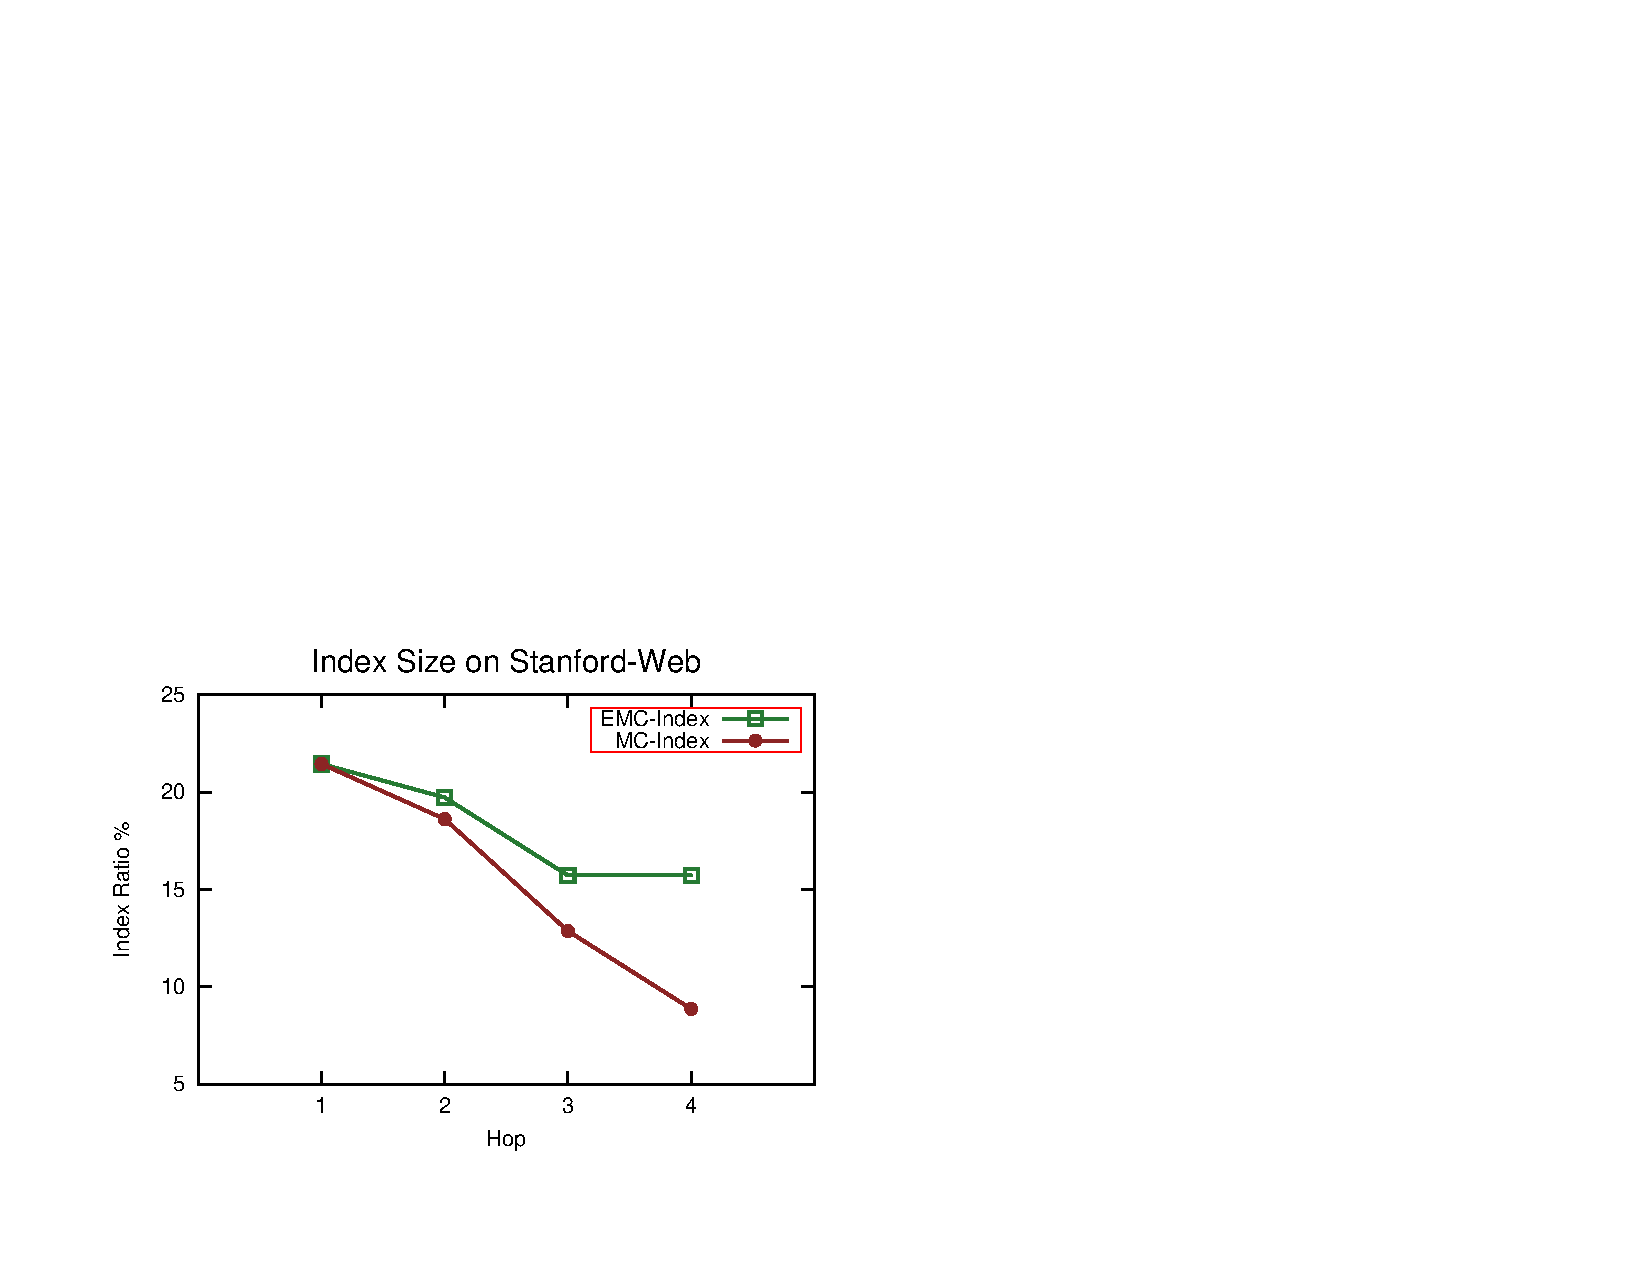
\includegraphics[width=\textwidth]{chapter3/exp/khopeffect/effectiveness/stanford_index_size.pdf}
  \caption{Index Size on Stanford-web}
\end{subfigure}
\caption{Index Construction Analysis for EMC and MC. (a) and (b) 
depict the index time for the Amazon and Stanford-web networks; 
(c) and (d) shows the index size for the Amazon and Stanford-web datasets}
\label{fig:index_analysis_emc_mc}
\end{figure*}


\subsection{Comparison between MC and EMC}
We first compare the effectiveness of the two DBIndex 
construction algorithms: MinHash Clustering (MC) and Estimated 
MinHash Clustering (EMC). We look at 
the index construction time, index sizes and query performance. 
All these experiments are conducted based on two real world datasets: 
Amazon and Stanford-web.For both datasets, we run a series of k-hop queries.\footnote{For the Stanford-web graph, which is directed,
the k-hop windows are directed k-hop windows where $u \in W(k)$ if there is a directed path
of at most $k$ hops from vertex $v$ to vertex $u$.
} For queries with hop count larger than 1, 
EMC uses 1-hop information for the initial clustering. 

\textbf{Index Construction. } Figs.~\ref{fig:index_analysis_emc_mc} 
(a) and (b) compare the index construction time between MC and EMC 
when we vary the windows from 1-hop to 4-hop for the Amazon and Stanford-web 
graphs respectively. To better understand the time difference, 
the construction time is split into two parts: 
the MinHash cost (EMC-hash or MC-hash) and the breadth-first-search traversal (to compute the k-hop window)  cost (EMC-bfs or MC-bfs). The results show the same trend 
for the two datasets. We made several observations.
First, as the number of hops increases, the indexing time increases as well. 
This is expected as a larger hop count results in a larger window size 
and the BFS and computation time increase correspondingly. 
Second, as the hop count increases, the difference between the
index time of EMC and that of MC widens. 
For instance, as shown in Figs.~\ref{fig:index_analysis_emc_mc}(a) and (b), for the 4-hop window queries, compared to MC, 
EMC can save $62\%$ and $66\%$ construction time for the Amazon and Stanford-Web datasets respectively.
EMC benefits from both the low MinHash cost and low BFS cost. 
From Figs.~\ref{fig:index_analysis_emc_mc} (a) and (b), 
we can see that the MinHash cost of MC increases as the number of hops 
increases, while that for EMC remains almost the same as the 1-hop case. 
This shows that the cost of MinHash becomes more significant for larger windows. 
Thus, using 1-hop clustering for larger hop counts reduces the MinHash cost 
in EMC. Similarly, as EMC saves on BFS cost for k-hop queries where $k > 1$, 
the BFS cost of EMC is much smaller than that of MC as well. 

\textbf{Index Size.} Figs.~\ref{fig:index_analysis_emc_mc} (c) and (d) 
present the effect of hop counts on the index size for the Amazon and Stanford-web 
datasets respectively. The y-axis shows the index ratio which is the index size over the original graph size. The insights we derive are: 
First, the index size is rather small compared to the original graph - it
varies from $3\%$ to $12\%$ of the original graph for the Amazon dataset 
and from $8\%$ to $22\%$ for the Stanford-web dataset. 
Second, the index size decreases as the number of hops increases. 
While this appears counter-intuitive initially, it is actually reasonable - a larger hop results in a bigger window, which leads
to more dense blocks. Third, the index ratio of EMC is slightly larger 
than that of MC for larger hop count. This indicates that MC can find more dense blocks 
than EMC to reduce the index size. Fourth, the index ratio on 
the Amazon dataset is much smaller than the ones on the Stanford-web dataset. 
This is because the Amazon dataset is undirected while the Stanford-web dataset
is directed. For the Stanford-web dataset, since we use directed k-hop windows, the window size is naturally smaller. 

\textbf{Query Performance.}       
Figs.~\ref{fig:khop_effective_query_time} (a) and (b)
present the query time of MC and EMC 
on the two datasets respectively 
as we vary the number of hops from 1 to 4.
To appreciate the benefits of an index-based scheme, we also implemented
a \emph{Non-indexed} algorithm which computes window aggregate by performing k-bounded breadth
first search for each vertex individually in real time.
In Figures~\ref{fig:khop_effective_query_time} (a) and (b),
the execution time shown on the y-axis is in log scale. The results show that the index-based 
schemes outperform the non-index approach by four orders of magnitude. 
For instance, for the 4-hop query over the Amazon graph, 
our algorithm is 13,000 times faster than the non-index approach. 
This confirms that it is necessary to have well-designed index support 
for efficient window query processing. By utilizing DBIndex, 
for these graphs with millions of edges, every aggregation query 
can be processed in just between 30ms to 100ms for the Amazon graph and 
between 60ms to 360ms for the Stanford-web graph. In addition, we can 
see that as the number of hops increases, the query time decreases. 
This is the case because a larger hop count eventually results in a larger
number of dense blocks where more (shared) computation can be salvaged. 
Furthermore, we can see that the query time of EMC is slightly longer 
than that of MC when the number of hops is large. This is expected as 
EMC does not cluster based on the complete window information; instead, it
uses only partial information derived from the 1-hop windows. 
However, the performance difference is quite small even for 4-hop queries- for
the Amazon dataset, the difference is only 20ms; and for the Stanford-web
graph, the difference is 35ms. 
For small number of hops, the time difference is even smaller. 
This performance penalty is acceptable as tens of milliseconds time 
difference will not affect user's experience.  As EMC is significantly more 
efficient than MC in index construction, EMC may still be a 
promising solution to many applications. As such, 
in the following sections, we adopt EMC for DBIndex in
our experimental evaluations.  
 
\begin{figure}[h]
\centering
\begin{subfigure}{0.48\linewidth}
\centering
  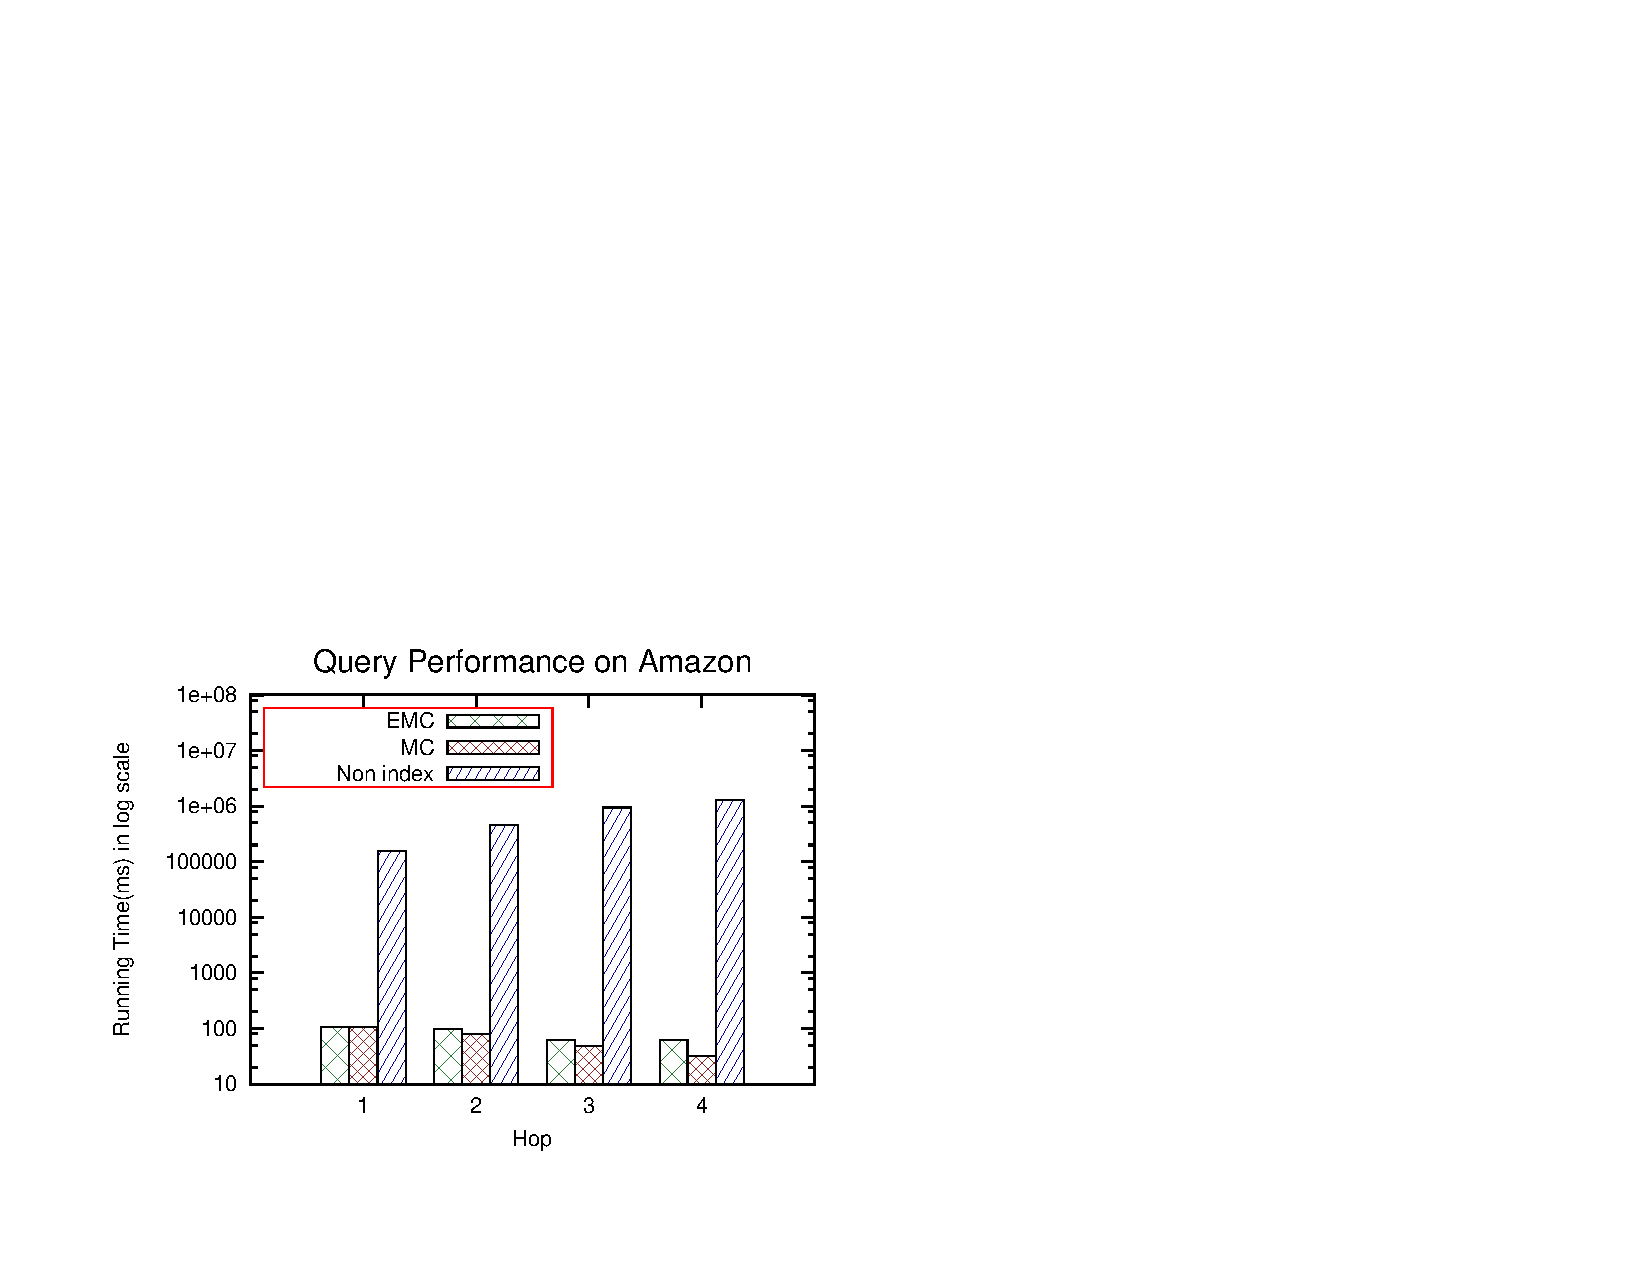
\includegraphics[width=\textwidth]{chapter3/exp/khopeffect/effectiveness/amazon_query_time.pdf}
  \caption{Amazon Graph}
\end{subfigure}%
\begin{subfigure}{0.48\linewidth}
\centering
  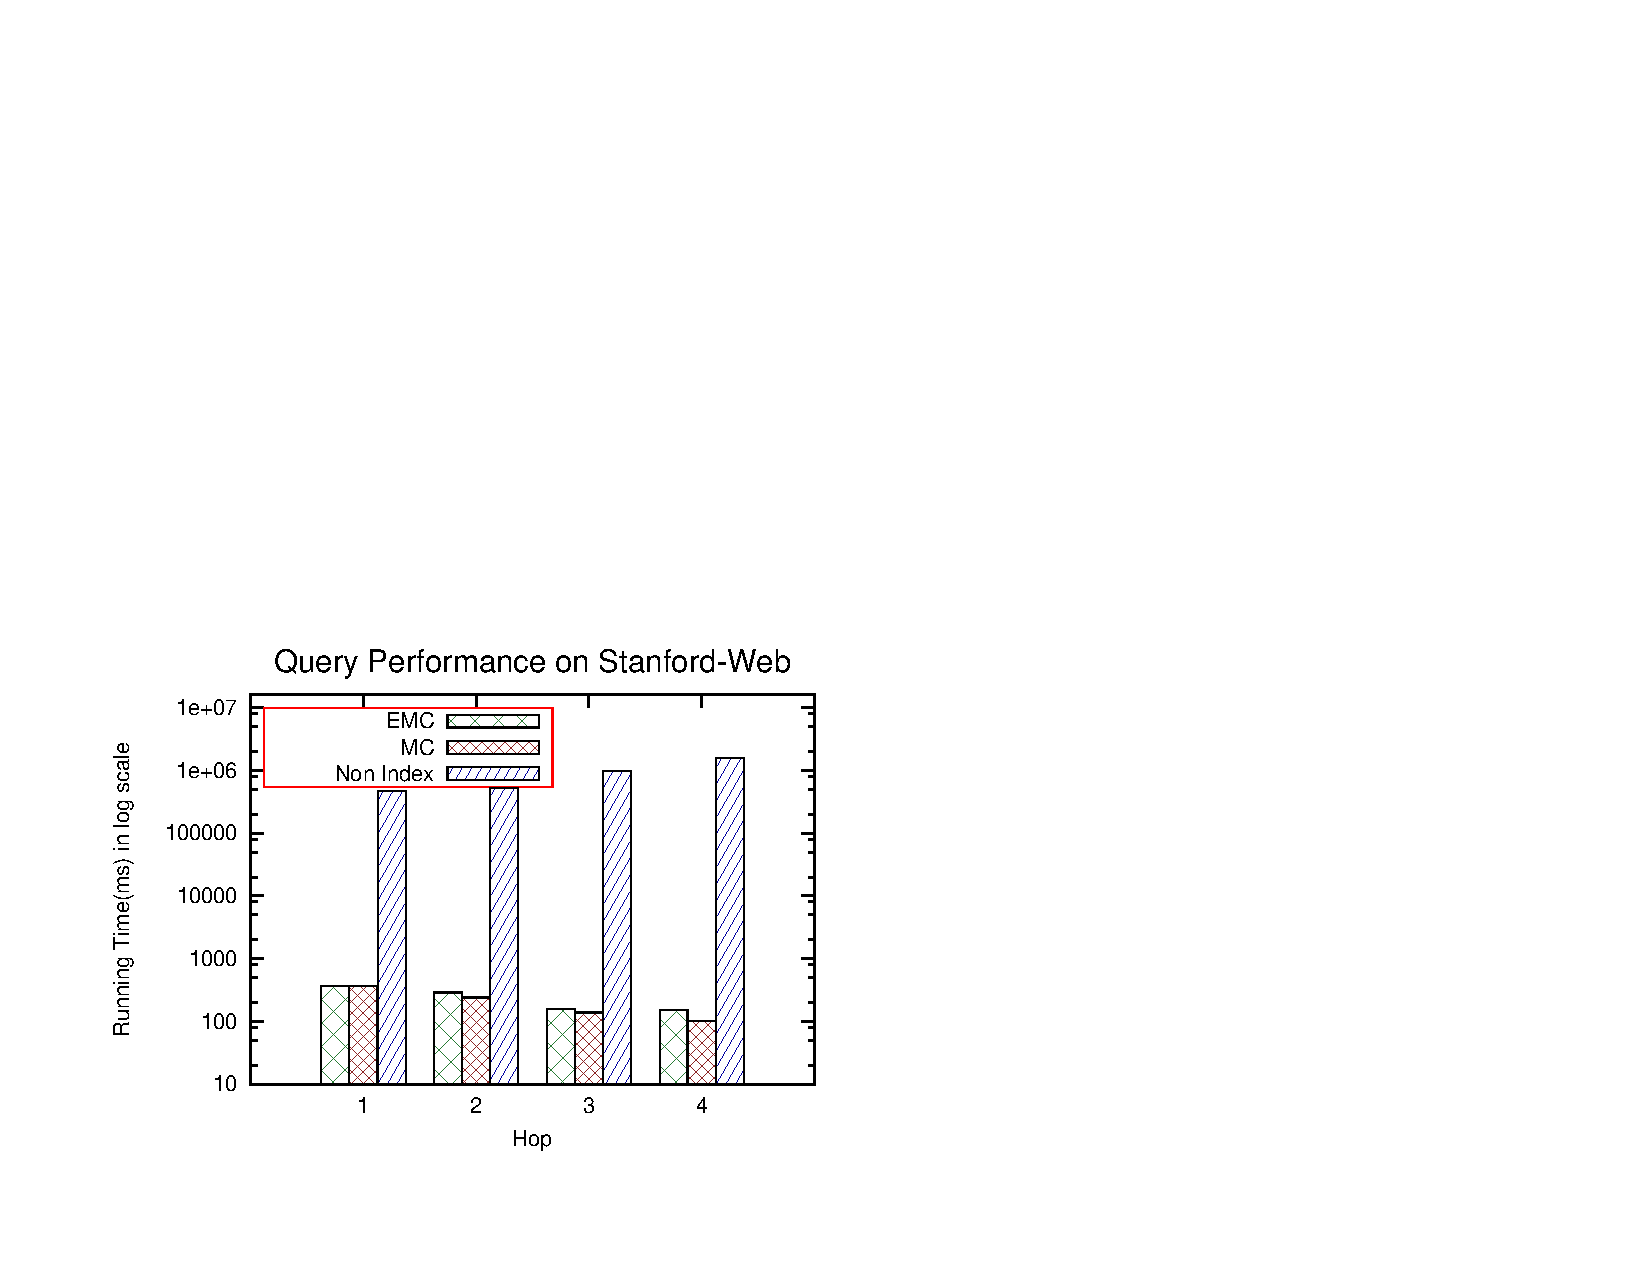
\includegraphics[width=\textwidth]{chapter3/exp/khopeffect/effectiveness/stanford_query_time.pdf}
  \caption{Stanford-web Graph}
\end{subfigure}
\caption{Query Performance Comparison of MC and EMC}
\label{fig:khop_effective_query_time}
\end{figure}

\subsection{Comparison between DBIndex and EAGR}

In this set of experiments, we compare DBIndex and 
EAGR \cite{mondal2014eagr} using both large-scale real 
and synthetic datasets. Like \cite{mondal2014eagr},
for each dataset, EAGR is run for 10 
iterations in the index construction.

\subsubsection{Real Datasets} 
We first study the index construction and 
query time performance of DBIndex and EAGR for 1-hop and 2-hop windows 
using 6 real datasets: DBLP, Youtube, Livejournal, Google, Pokec and Orkut. 
The results for 1-hop window and 2-hop window are presented
in Figs.~\ref{fig:1-hop-real} and~\ref{fig:2-hop-real} 
respectively. 
As shown in Figs.~\ref{fig:1-hop-real}(a) and~\ref{fig:2-hop-real}(a), both DBIndex and EAGR can build the index for all
the real datasets for 1-hop but EAGR ran out of the memory for 2-hop window queries on LiveJournal and Orkut datasets. This further confirms that EAGR incurs 
high memory usage as it needs to build the FPT and 
maintain the vertex-window mapping information. We also observe that 
DBIndex is significantly faster than EAGR in index creation. 
We emphasize that the time is shown in logarithmic scale. 
For instance, for Orkut dataset, EAGR takes 4 hours to build the index 
while DBIndex only takes 33 minutes. 

Fig.~\ref{fig:1-hop-real} (b) and Fig.~\ref{fig:2-hop-real} (b) 
show the query performance for 1-hop and 2-hop queries respectively. 
The results indicate that the query performance is comparable. 
For most of the datasets, DBIndex is faster than EAGR.
In some datasets (e.g. Orkut and Pokec), DBIndex performs 30\% faster than the EAGR. 
We see that, for 1-hop queries on 
Youtube and LiveJournal datasets and 2-hop queries on Youtube dataset, DBIndex is slightly slower than EAGR. We observe 
that these datasets are very sparse graphs where the intersections among windows are naturally small. For very sparse graphs, 
both DBIndex and EAGR are unable to find much computation sharing. In this case, the performance of DBIndex and EAGR is very close. For instance, in the worse case for livejournal, DBIndex is 9\% slower than EAGR where the actual time difference remains tens of millionseconds.    
 
Another insight we gain is that as expected, compared to Fig.~\ref{fig:1-hop-real} (b), 
2-hop query runs faster for both algorithms. This is because there is more computation sharing for 2-hop window query. 

In summary, 
DBIndex takes much shorter time to build but offers comparable, if not much faster, query 
performance than EAGR.


\begin{figure}[h]
\centering
\begin{subfigure}{0.48\linewidth}
  \centering
  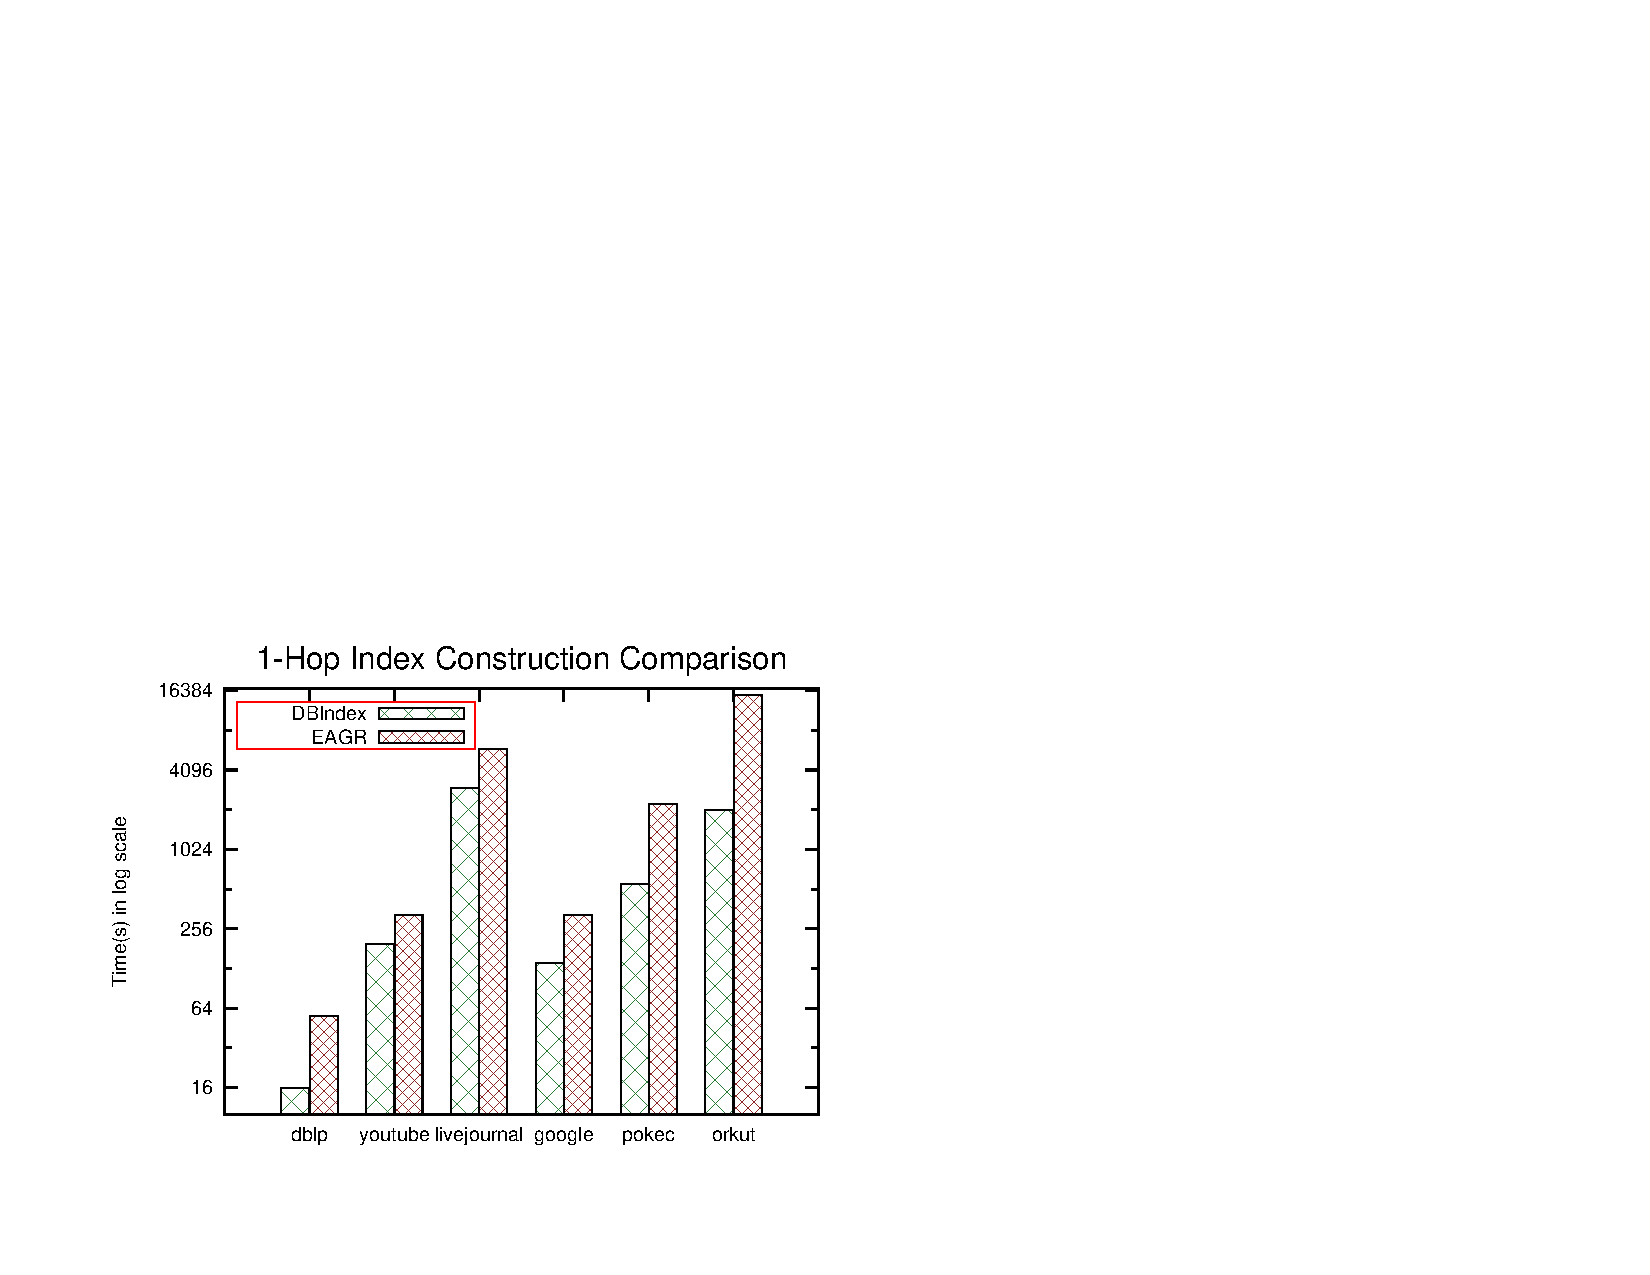
\includegraphics[width=\textwidth]{chapter3/exp/khopeffect/real_data/real_index_time_h1.pdf}
  \caption{Index Construction}
\end{subfigure} \begin{subfigure}{0.48\linewidth}
  \centering
  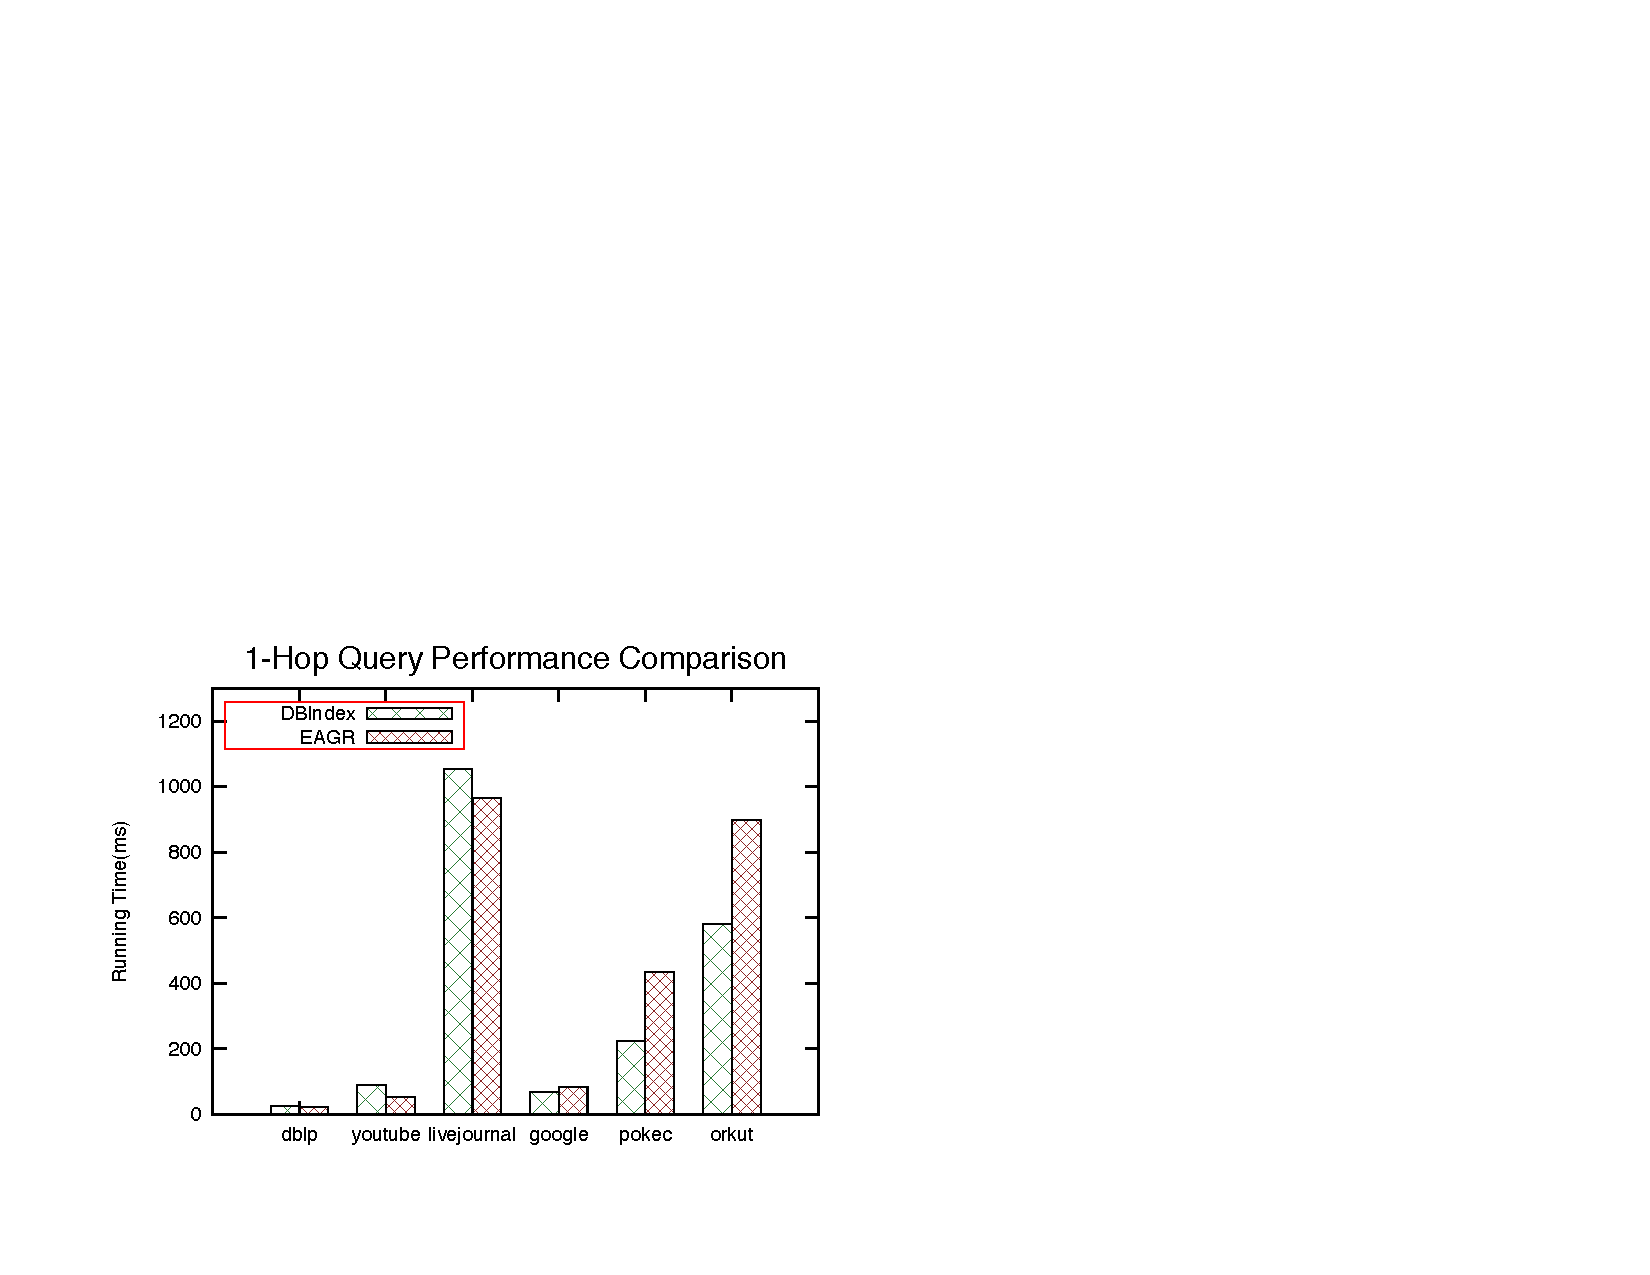
\includegraphics[width=\textwidth]{chapter3/exp/khopeffect/real_data/real_query_time_h1.pdf}
  \caption{Query Performance}
\end{subfigure}%
\caption{Comparison between DBIndex and EAGR  for 1-hop query}
\label{fig:1-hop-real}
\end{figure}

\begin{figure}[h]
\centering
\begin{subfigure}{0.48\linewidth}
  \centering
  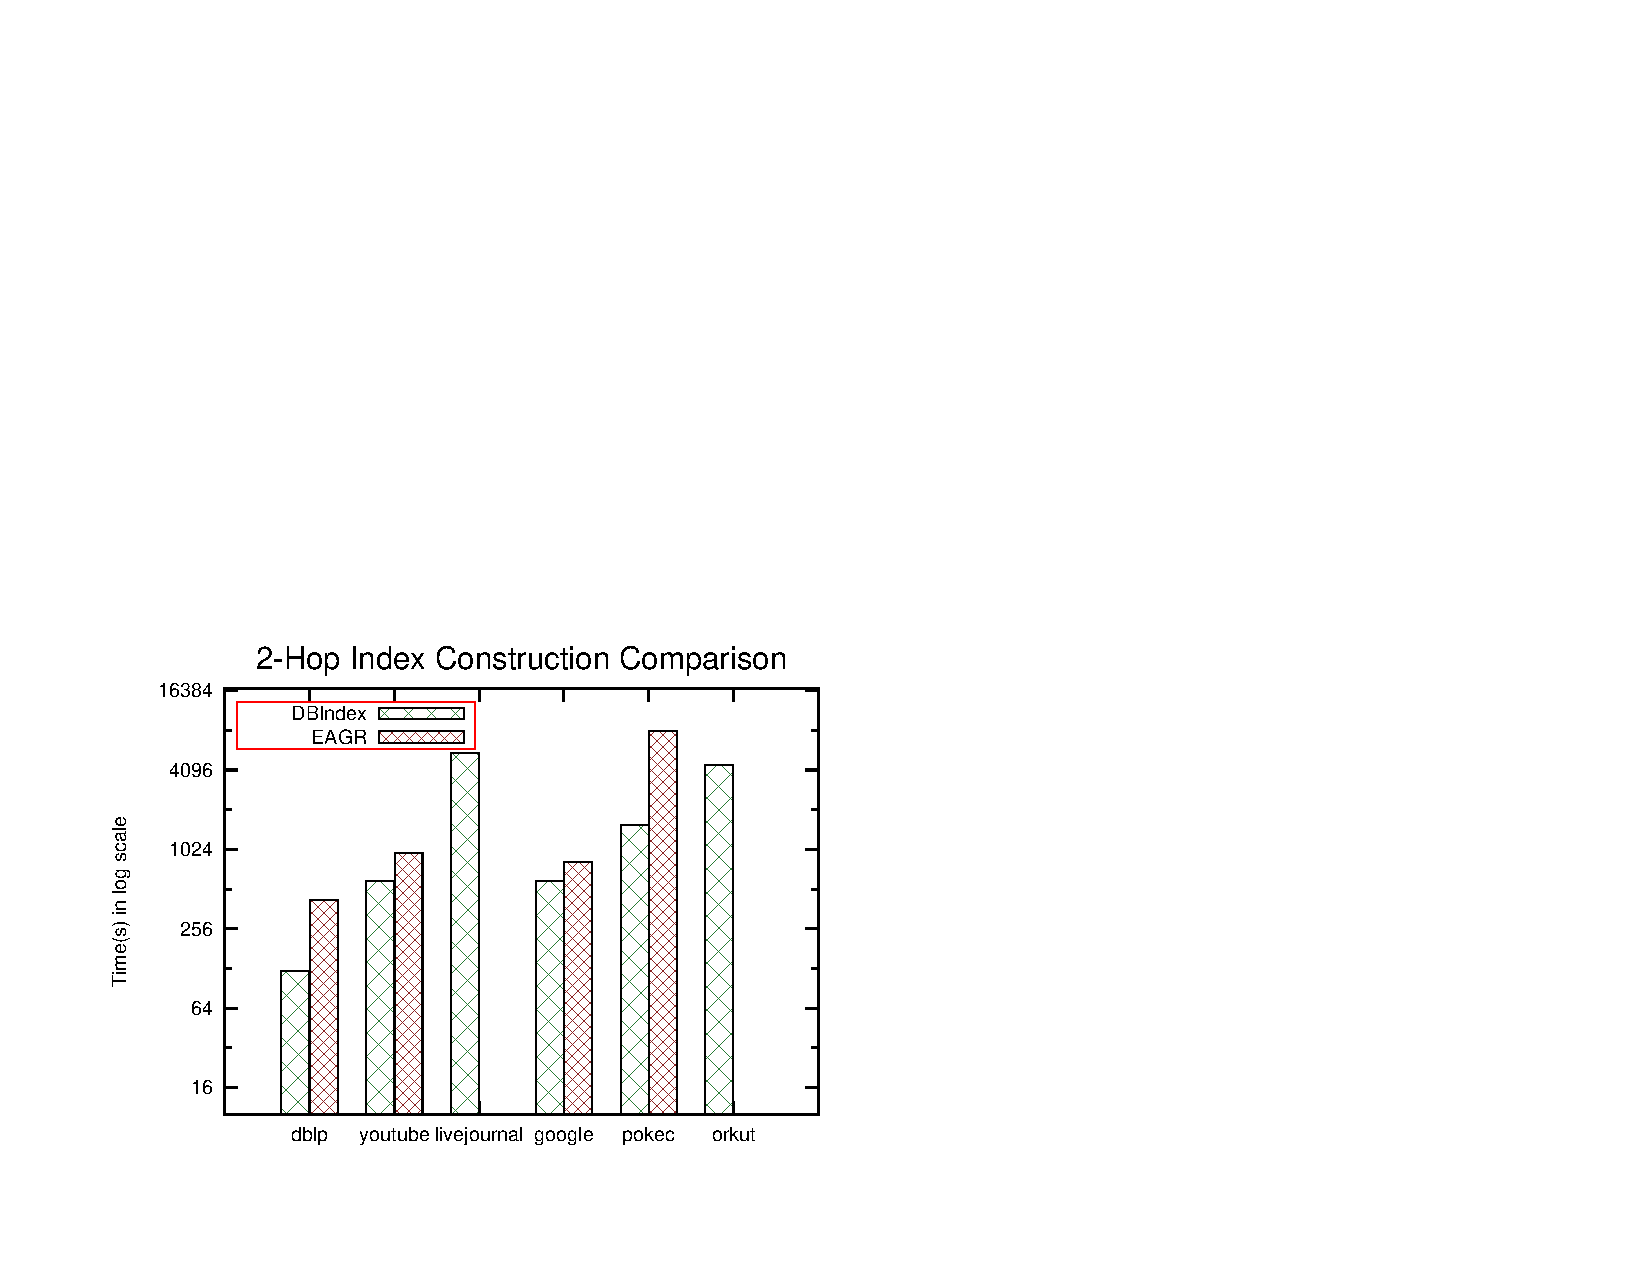
\includegraphics[width=\textwidth]{chapter3/exp/khopeffect/real_data/real_index_time_h2.pdf}
  \caption{Index Construction}
\end{subfigure}
\begin{subfigure}{0.48\linewidth}
  \centering
  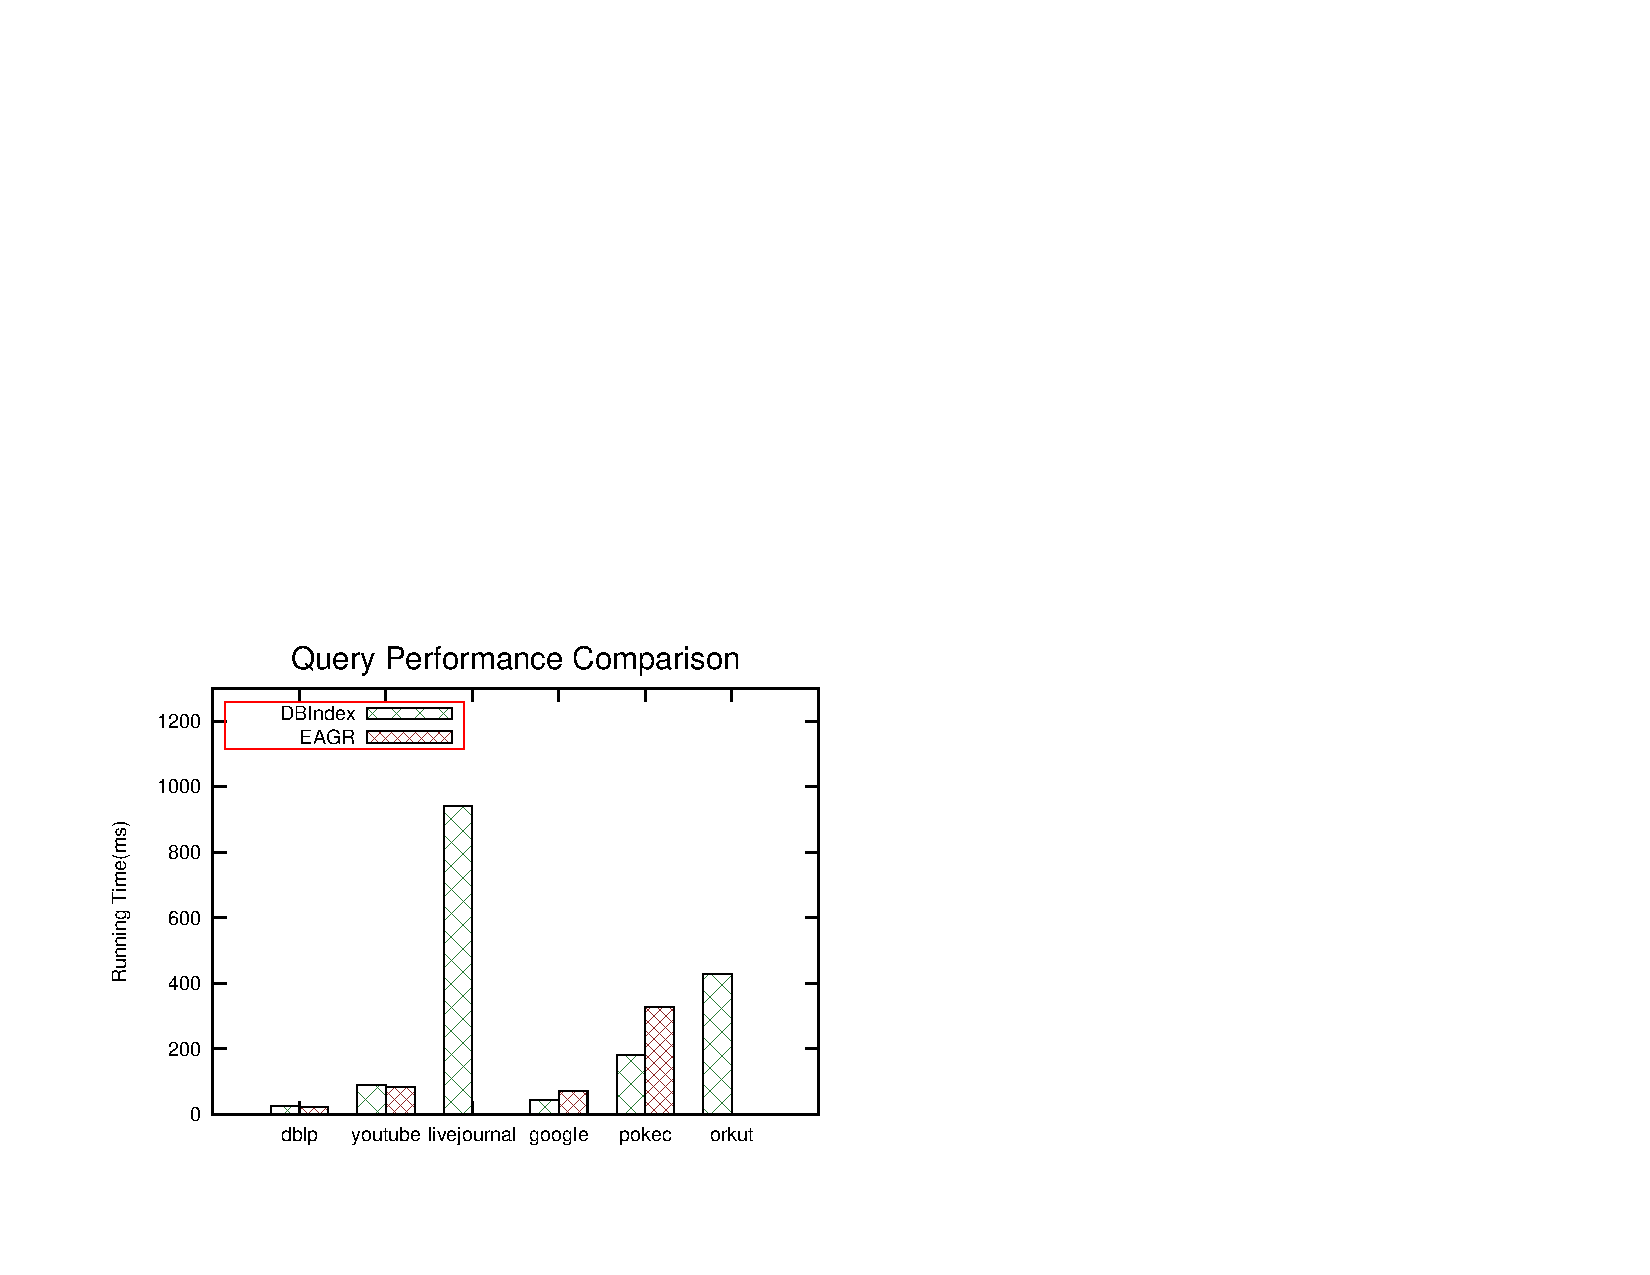
\includegraphics[width=\textwidth]{chapter3/exp/khopeffect/real_data/real_query_time_h2.pdf}
  \caption{Query Performance}
\end{subfigure}
\caption{Comparison between DBIndex and EAGR for 2-hop query}
\label{fig:2-hop-real}
\end{figure}


\subsubsection{Synthetic Datasets}
To study the scalability of DBIndex under large-scale networks, 
we generated synthetic datasets using the SNAP generator. 

% streching from 2M vertices to 10M vertices. To see the scalability of our index, we perform extensive tests from both degree and vertex angle.  All data are generated from SNAP\footnote{http://snap.stanford.edu/snap/download.html} graph generator program. We use EAGR as a comparison method. We reported our findings below:

\textbf{Impact of Number of Vertices.} First, we study how the performance 
changes when we fix the degree \footnote{Degree means average degree of the graph. The generated graph is of Erdos-Renyi model } at 10 and vary the number of vertices from 
2M to 10M. Figs.~\ref{fig:khop_d10_h1} (a) and (b) show
the execution time for index construction and query performance respectively.
From the results, we can see that DBIndex outperforms EAGR in
both index construction and query performance. For the graph with 
10M vertices and 100M edges, the DBIndex query time is less than 
450 milliseconds. 
%The increment of DBIndex query with respect to vertex is also steady. 
Moroever, when the number of vertices changes from 2M to 10M, 
the query performance only increases 3 times. This shows that
DBIndex is not only scalable, but offers acceptable performance..   

\begin{figure}[t]
\centering
\begin{subfigure}{0.48\linewidth}
  \centering
  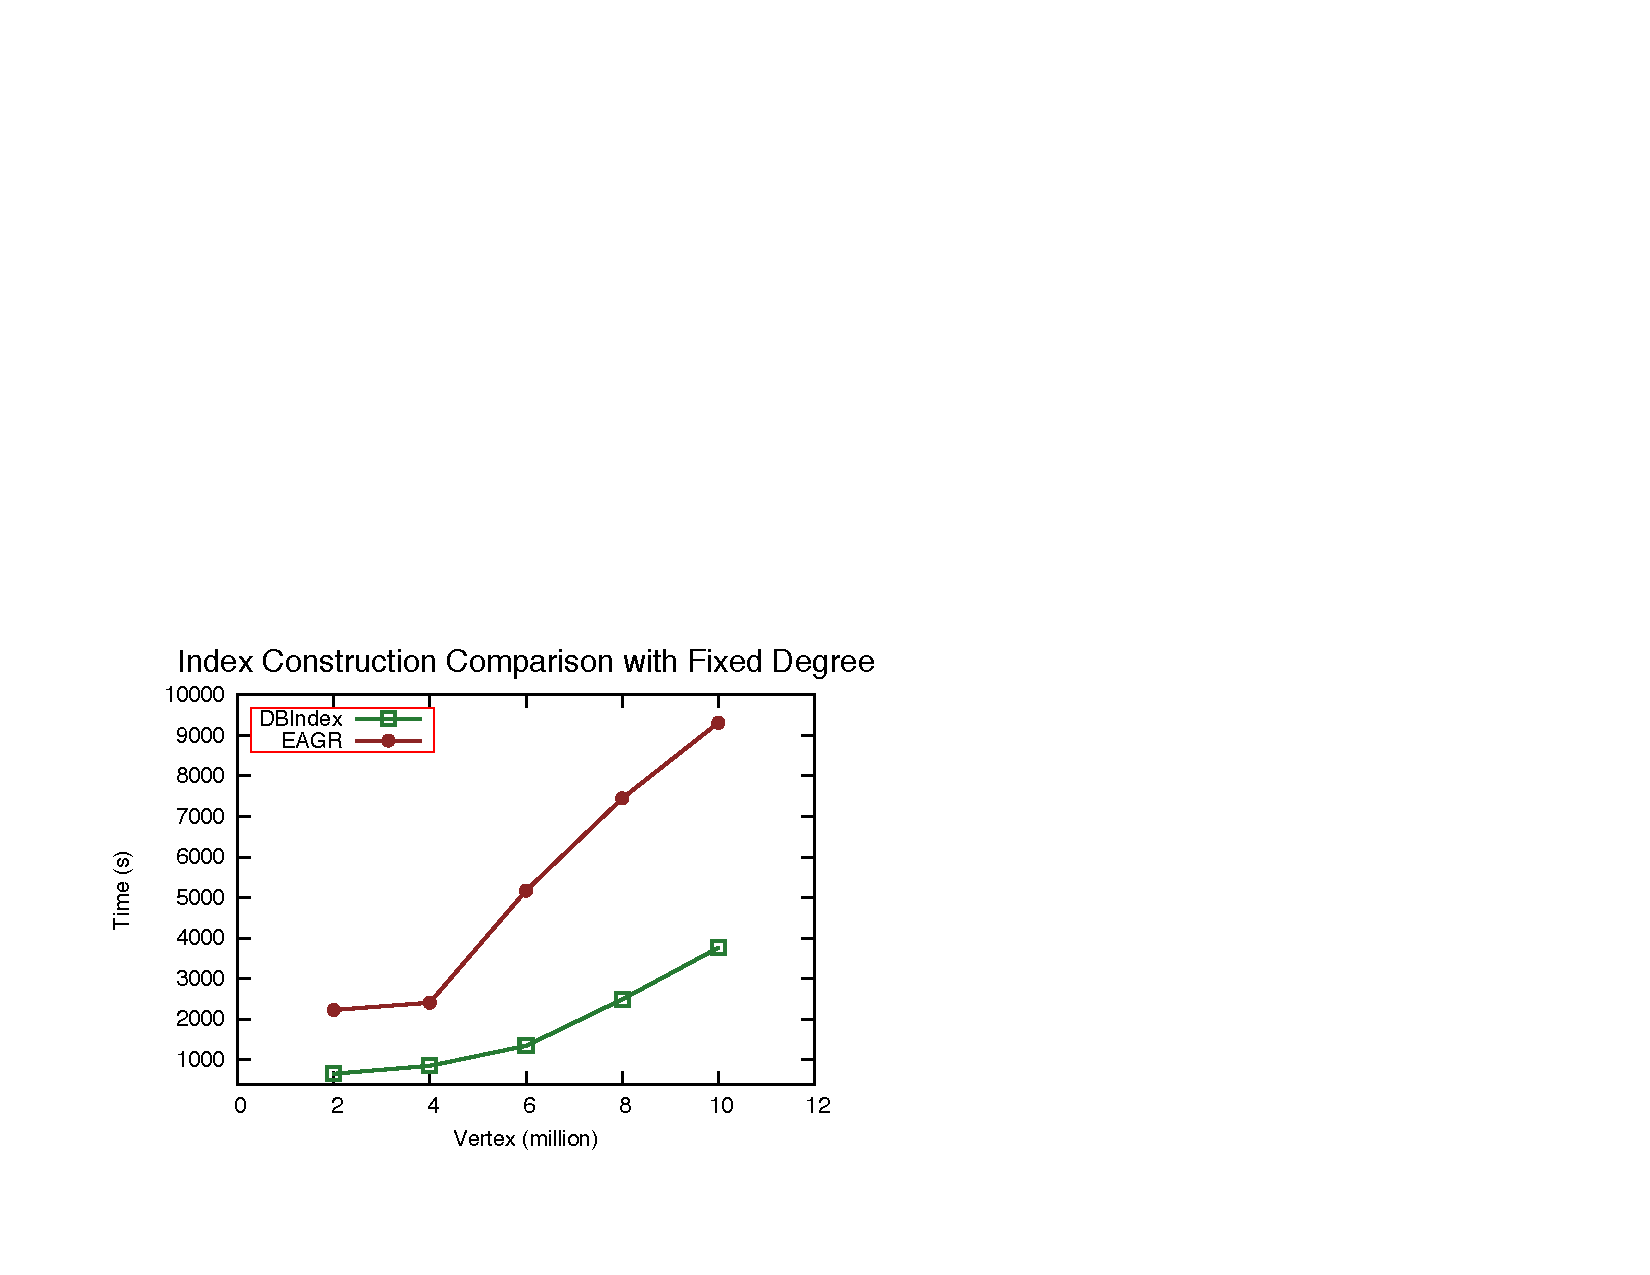
\includegraphics[width=\textwidth]{chapter3/exp/khopeffect/scalability/d10h1_index.pdf}
  \caption{Index Construction}
\end{subfigure}
\begin{subfigure}{0.48\linewidth}
  \centering
  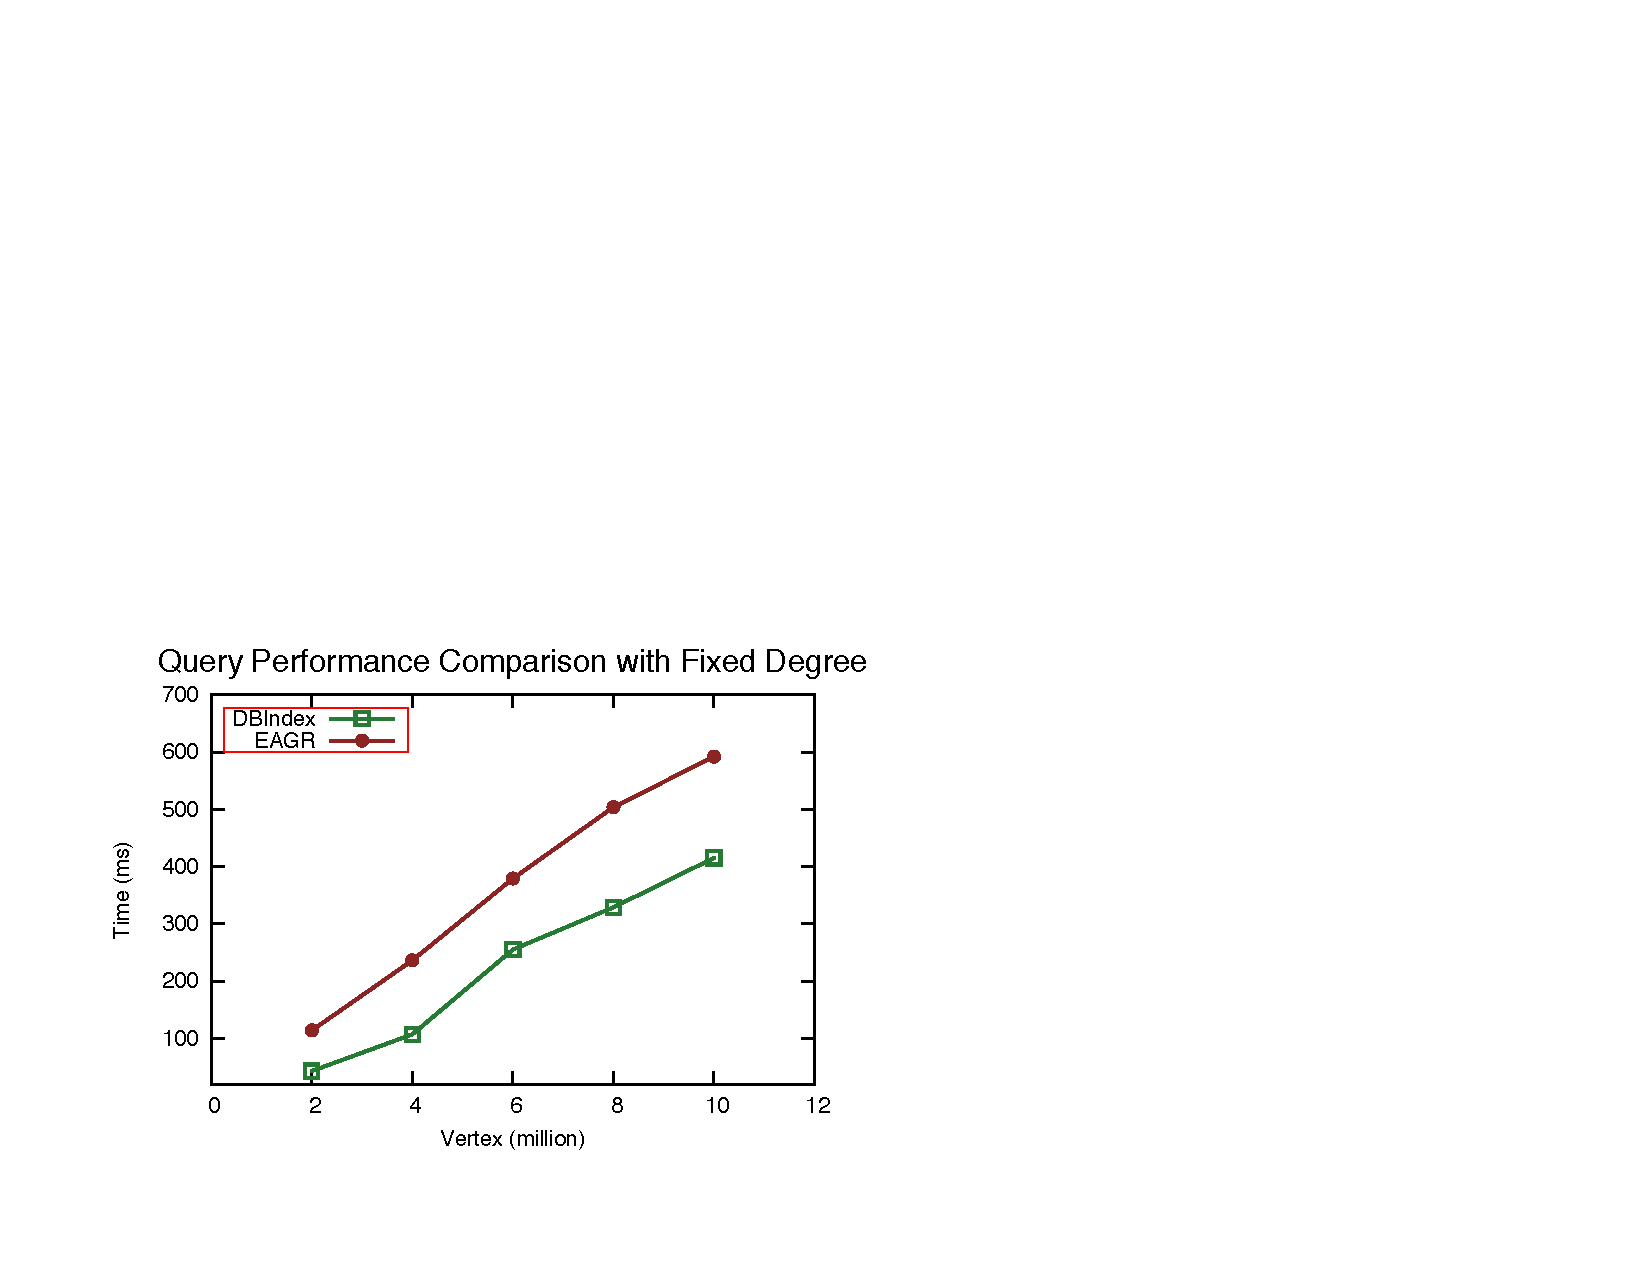
\includegraphics[width=\textwidth]{chapter3/exp/khopeffect/scalability/d10h1_time.pdf}
  \caption{Query Performance}
\end{subfigure}%
\caption{Impact of number of vertices }
\label{fig:khop_d10_h1}
\end{figure}

\begin{figure}[t]
\centering
\begin{subfigure}{0.46\linewidth}
  \centering
  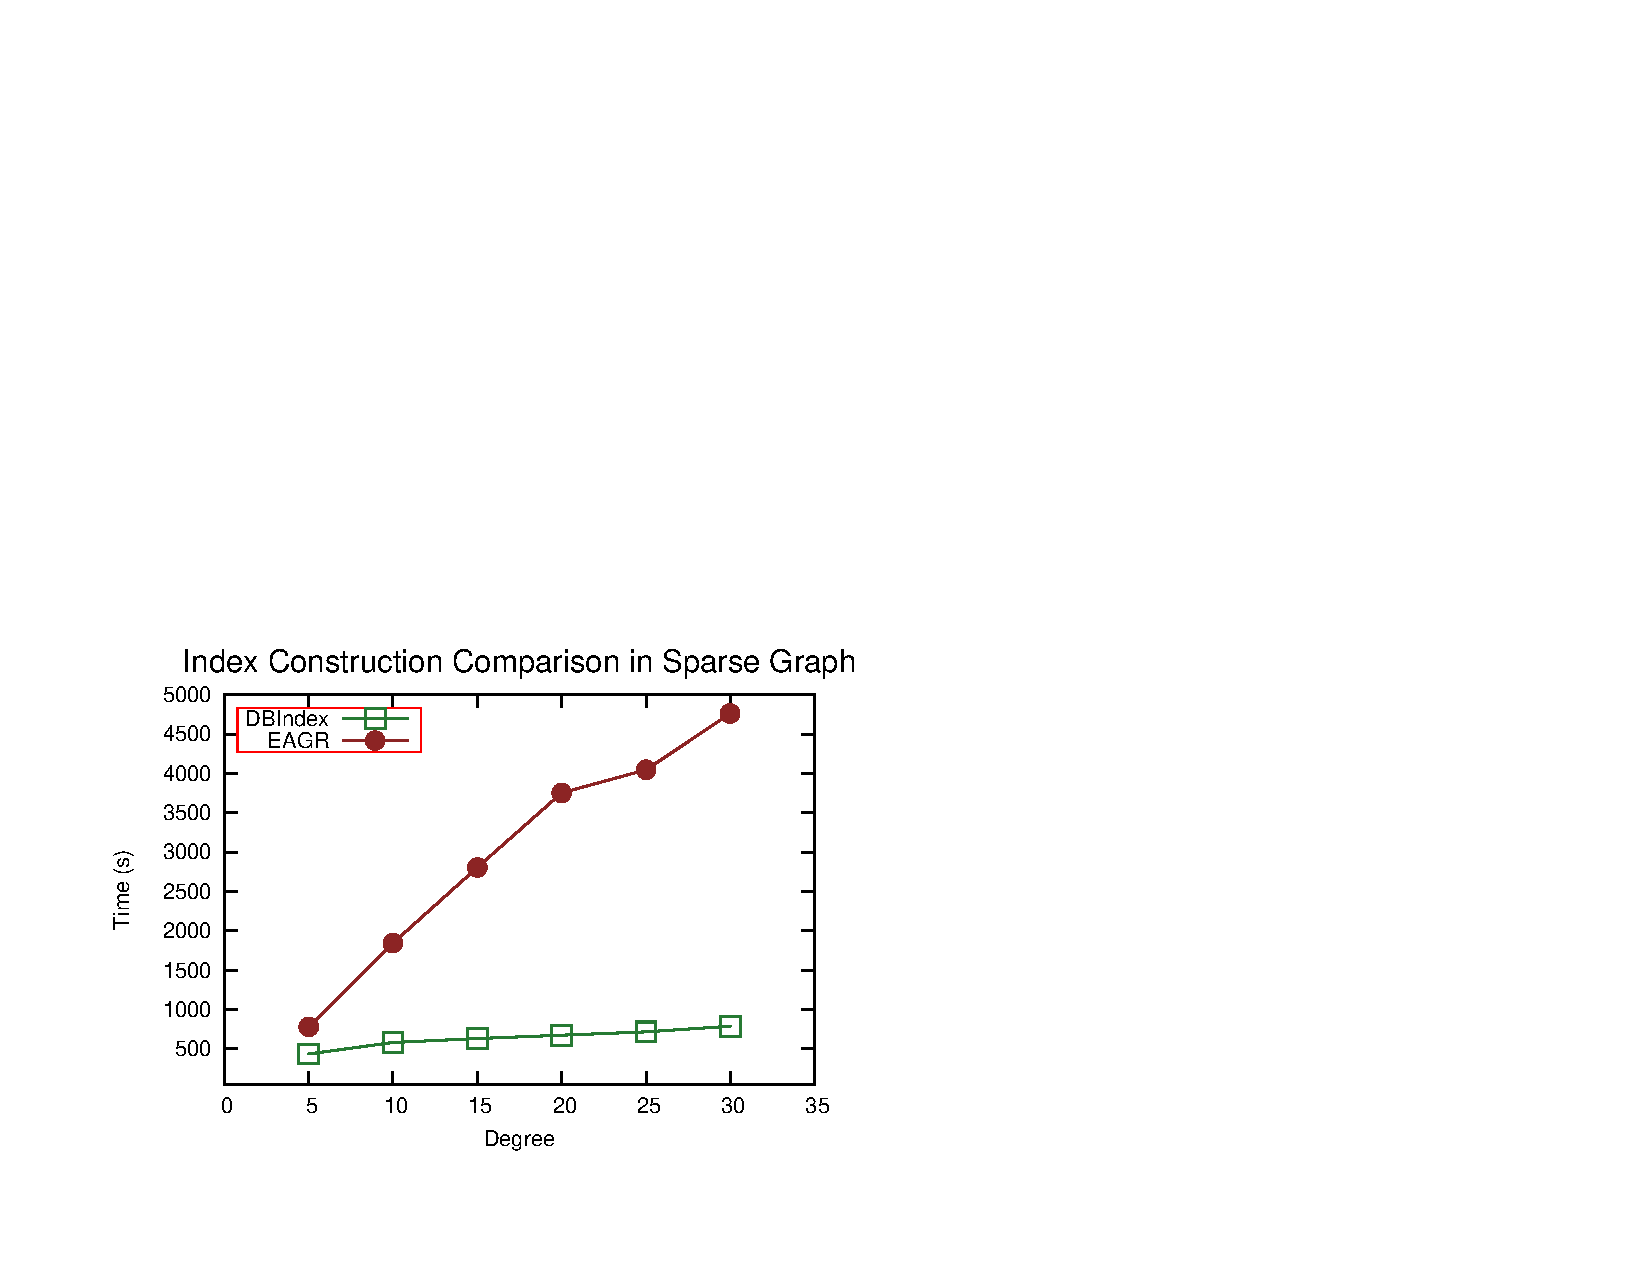
\includegraphics[width=\textwidth]{chapter3/exp/khopeffect/scalability/varyd_index_2M.pdf}
  \caption{Index Construction}
\end{subfigure}
\begin{subfigure}{0.50\linewidth}
  \centering
  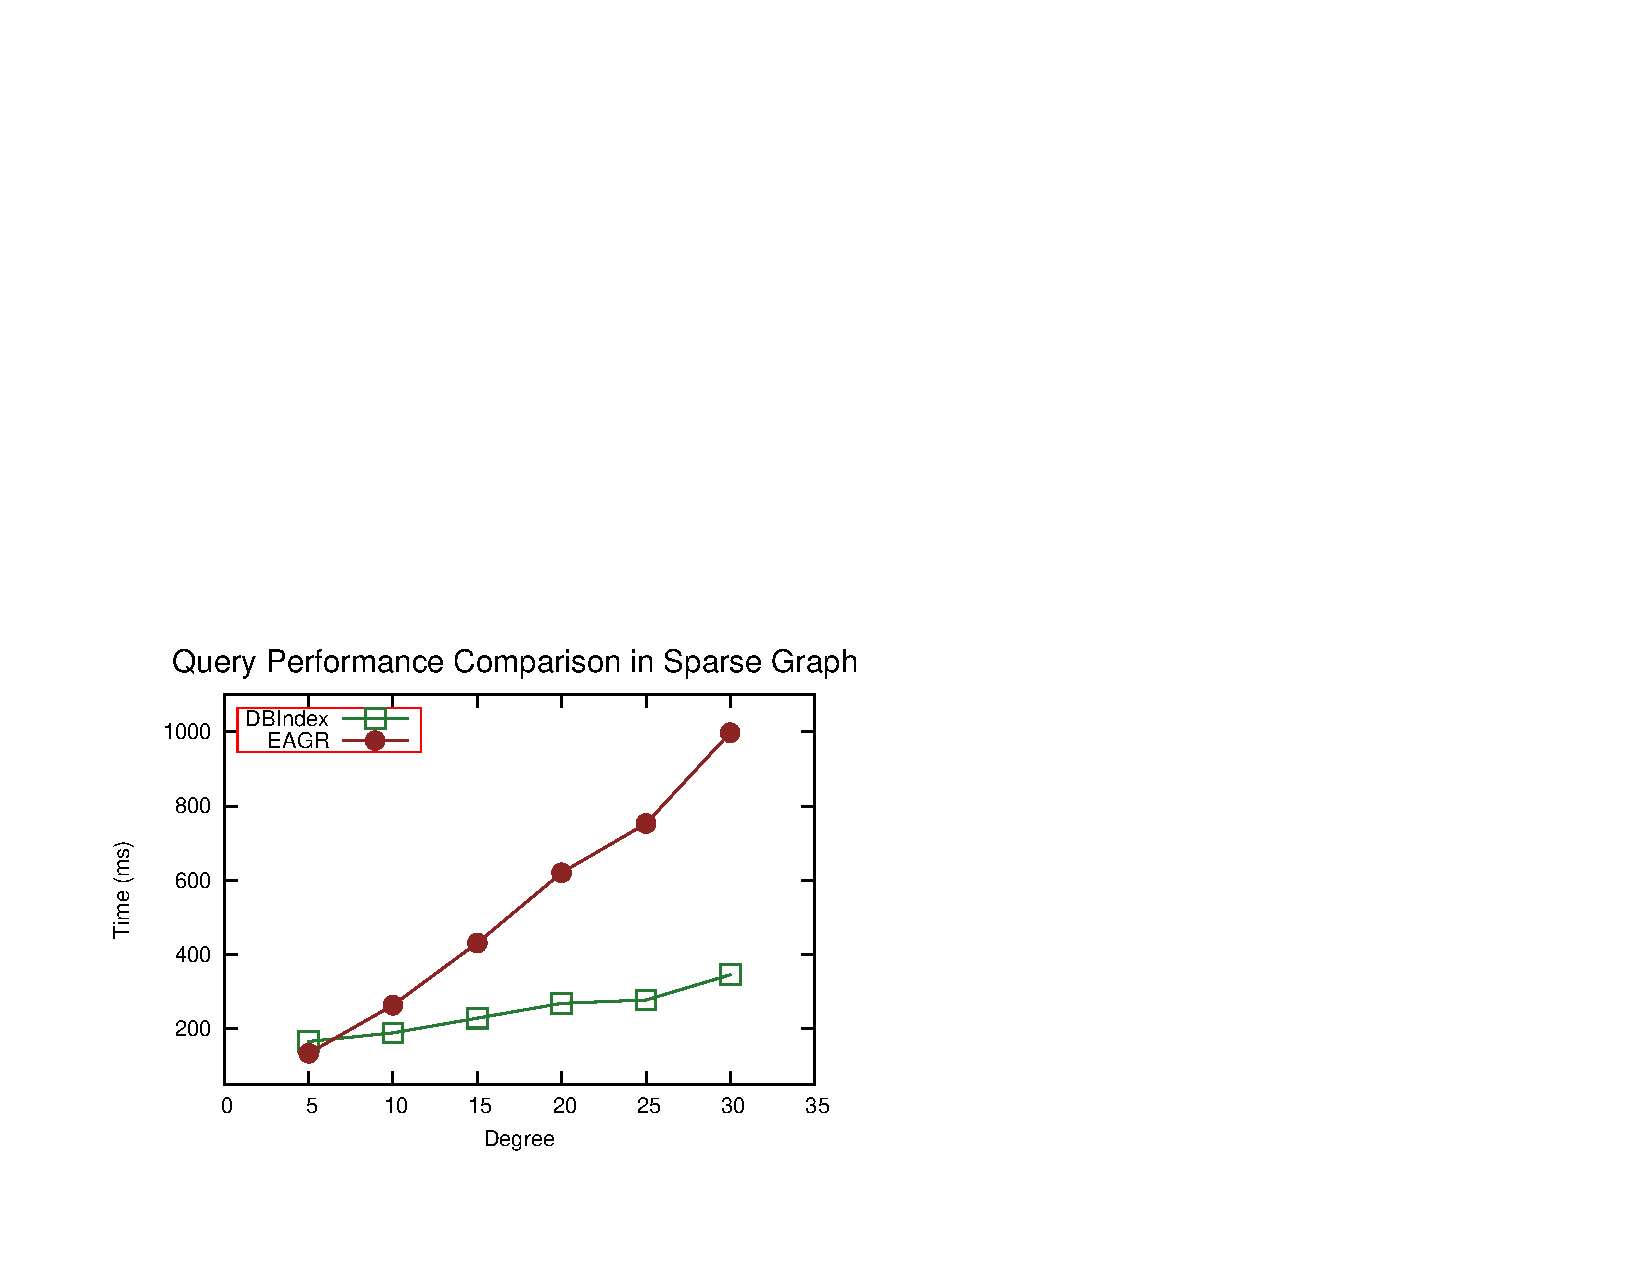
\includegraphics[width=\textwidth]{chapter3/exp/khopeffect/scalability/varyd_query_2M.pdf}
  \caption{Query Performance}
\end{subfigure}
\begin{subfigure}{0.50\linewidth}
  \centering
  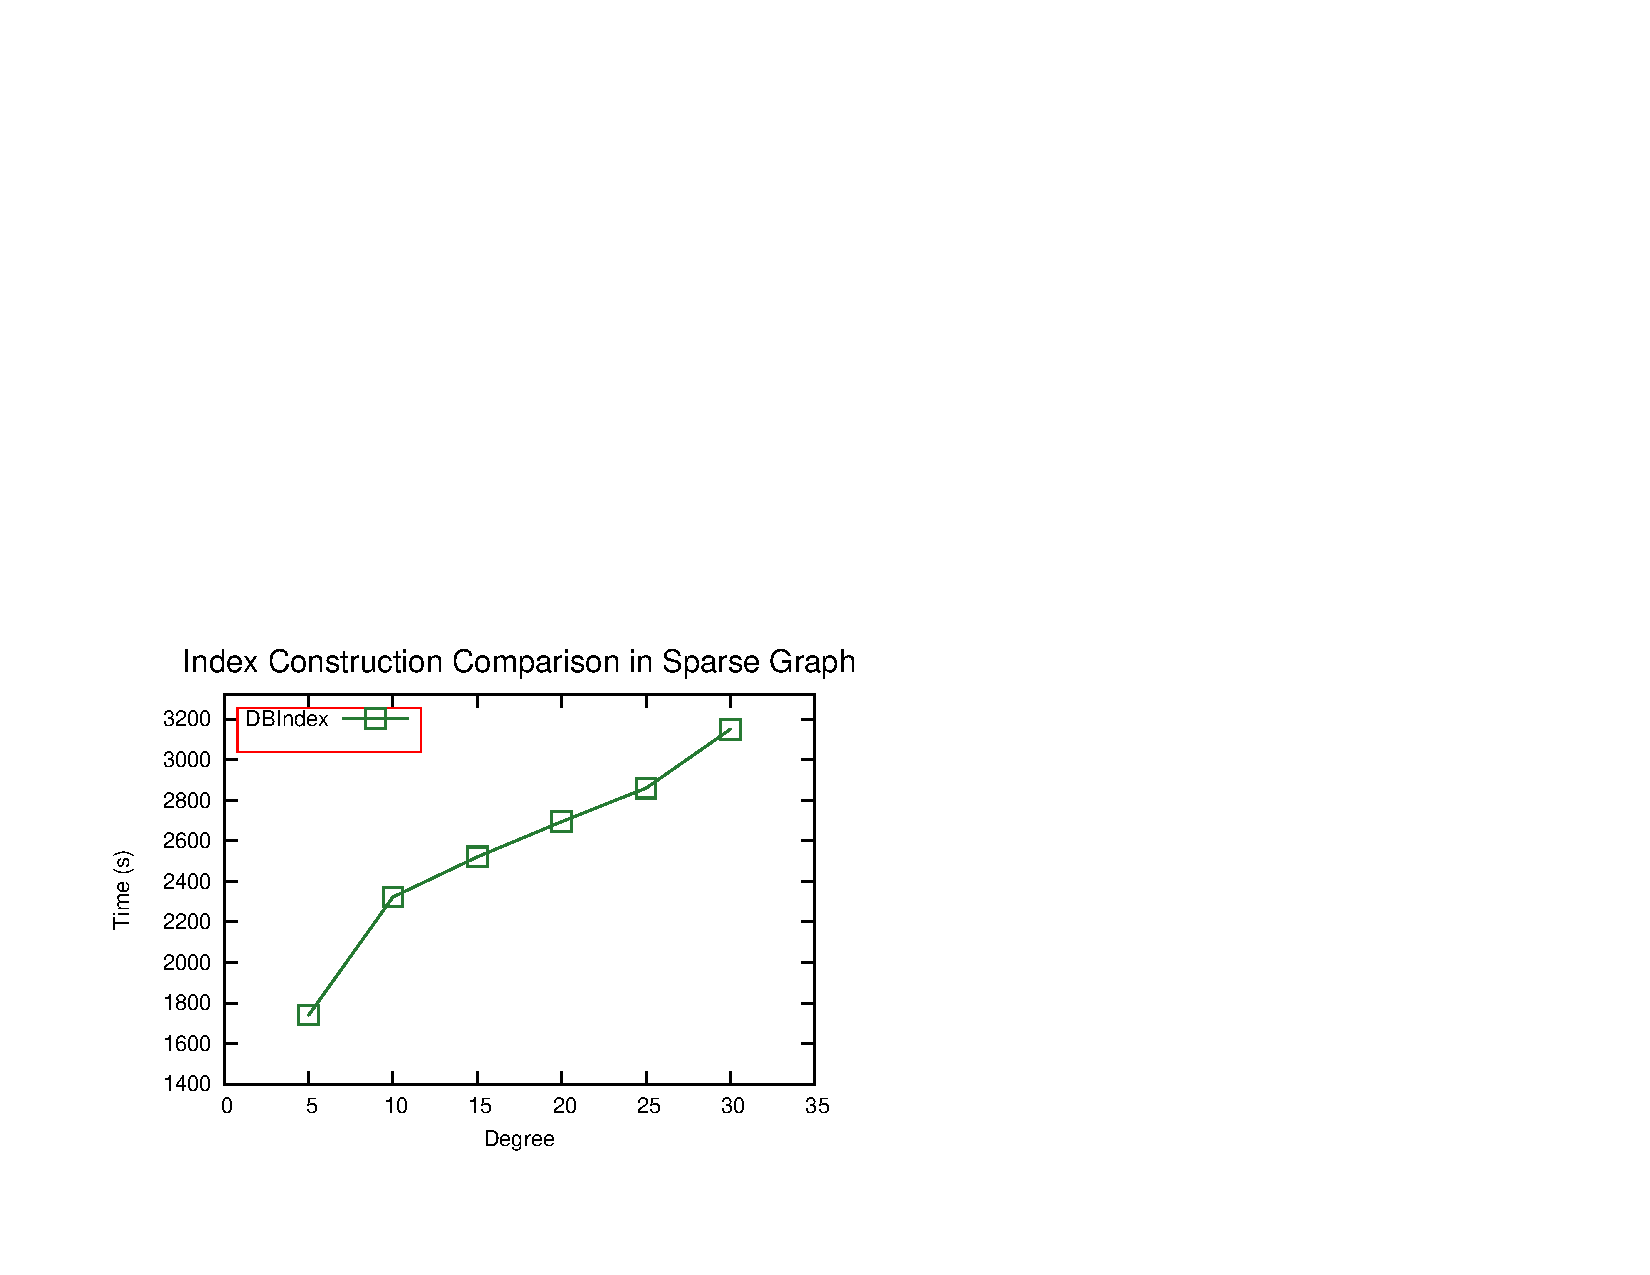
\includegraphics[width=\textwidth]{chapter3/exp/khopeffect/scalability/varyd_index_2M_h2.pdf}
  \caption{Index Construction}
\end{subfigure}
\begin{subfigure}{0.46\linewidth}
  \centering
  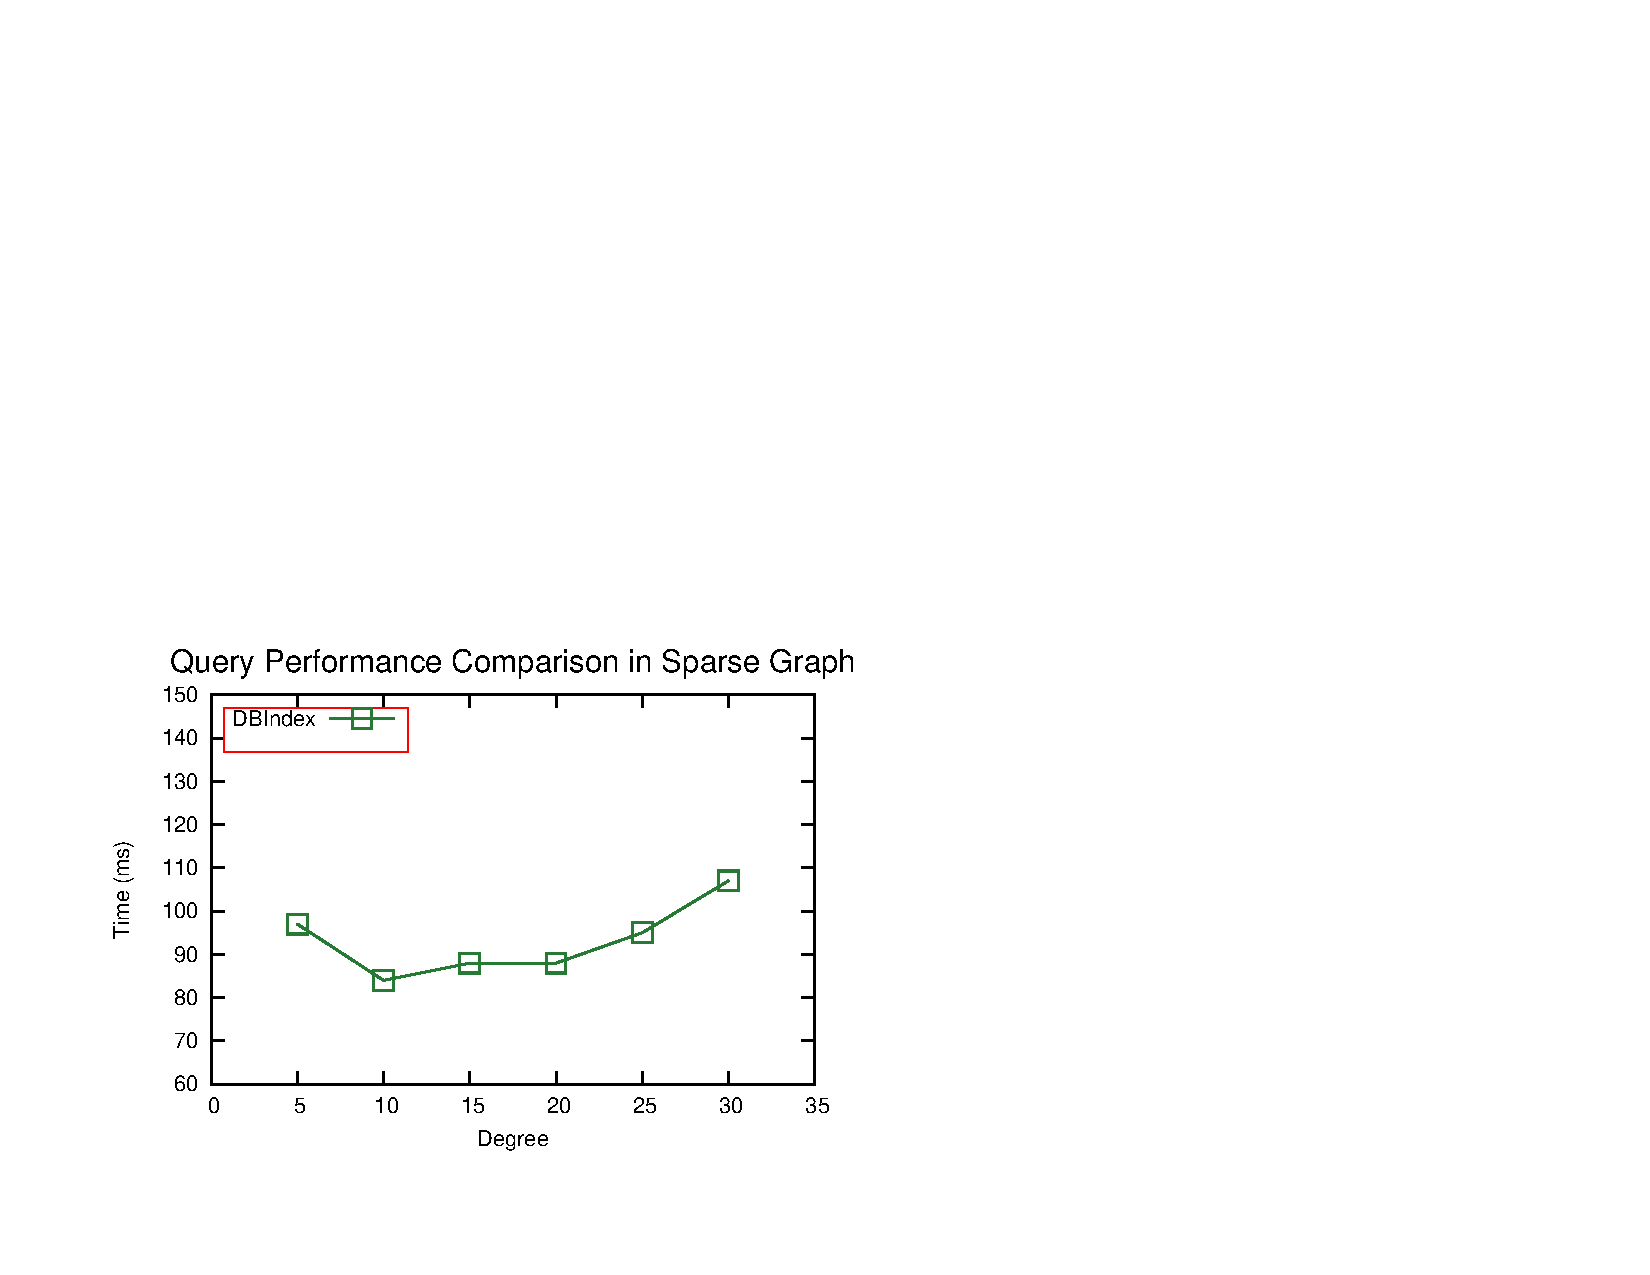
\includegraphics[width=\textwidth]{chapter3/exp/khopeffect/scalability/varyd_query_2M_h2.pdf}
  \caption{Query Performance}
\end{subfigure}
\caption{Impact of Degree over Sparse Graphs over 2M vertices. (a) and (b) are the results for 1-hop query; (c) and (d) are the results for 2-hop query. }
\label{fig:khop_v2m}
\end{figure}

\textbf{Impact of Degree over Sparse Graphs.} Our proposed DBIndex is effective when there is significant overlap between windows of neigboring nodes. As such, it is interesting to study how it performs for sparse graph where the nodes may not share many common neigbors. So, in these experiments, 
we study the impact of degree when the graph is relatively sparse.
We fix the number vertices of 2M and vary the vertex degree from 5 to 30. 
Figs.~\ref{fig:khop_v2m} (a) and (c) present the results 
on index construction for 1-hop and 2-hop queries respectively. 
For 1-hop queries, as degree increases, the time for index
construction also increases. 
However, the index creation time of DBIndex increases much 
slower than EAGR. This is because EAGR incurs relatively more 
overhead to handle multiple FPT creation and reconstruction. 
For 2-hop queries, EAGR failed to run. This is because even for 
a degree 5 sparse graph, the initial vertex-mapping can be as large 
as 90GB in a linked list manner, which exceeds the available memory. 
Note that the size becomes even larger when it is stored in a matrix manner.
Therefore, we can only show the results of DBIndex. 
In Fig.~\ref{fig:khop_v2m} (c), indexing time of DBIndex increases as the 
degree increases. This is expected as a bigger degree  
increases the overhead of graph traversal time to collect the window. 


Fig.~\ref{fig:khop_v2m} (b) and (d)
show the results on query time 
for 1-hop and 2-hop queries respectively. 
We observe a similar pattern for the index construction time:
for 1-hop queries, the query time increases with increasing degree
but at a much slower rate than EAGR; for 2-hop queries, we observe in Fig.~\ref{fig:khop_v2m} (d) that the
query performance of DBIndex hovers around 100ms, which is much 
smaller than that of 1-hop query performance. 
This is because there are more dense blocks in the 2-hop case, 
in which case the query time can be faster compared to the 1-hop case. 

\textbf{Impact of Degree over Dense Graphs.} We study the 
impact of degree over very dense graphs with 200k vertices 
when the degree changes from 80 to 200. 
Figs.~\ref{fig:khop_v200k} (a) and (c) show
the execution time for index construction 
for 1-hop and 2-hop queries respectively. From the results, 
we can see that DBIndex performs well for dense graphs as well. 
As the degree increases, EAGR's performance degrades much faster than DBIndex. For 2-hop queries,
as shown in Figs.~\ref{fig:khop_v200k} (b) and (d), EAGR is only able to work on 
the dataset with degree 80 due to the memory issue. 
Even though the number of vertices is relatively small (only 200k), 
the number of edges is very large when the degree becomes big 
(e.g. 40M edges with degree of 200). 

Figs.~\ref{fig:khop_v200k} 
(b) and (d) show the results on query performance 
for 1-hop and 2-hop queries respectively. 
The results are consistent with that for sparse graphs
- DBIndex is superior over EAGR. 

In summary, the insight we obtain is that the scalability of EAGR 
is highly limited by its approach to build the index over 
the vertex-window mapping information. EAGR is limited 
by two factors: the graph size and the number of hops. 
DBIndex achieves better scalability as it does not need to 
create a large amount of intermediate data in memory. 

\begin{figure}[h]
\centering
\begin{subfigure}{0.48\linewidth}
  \centering
  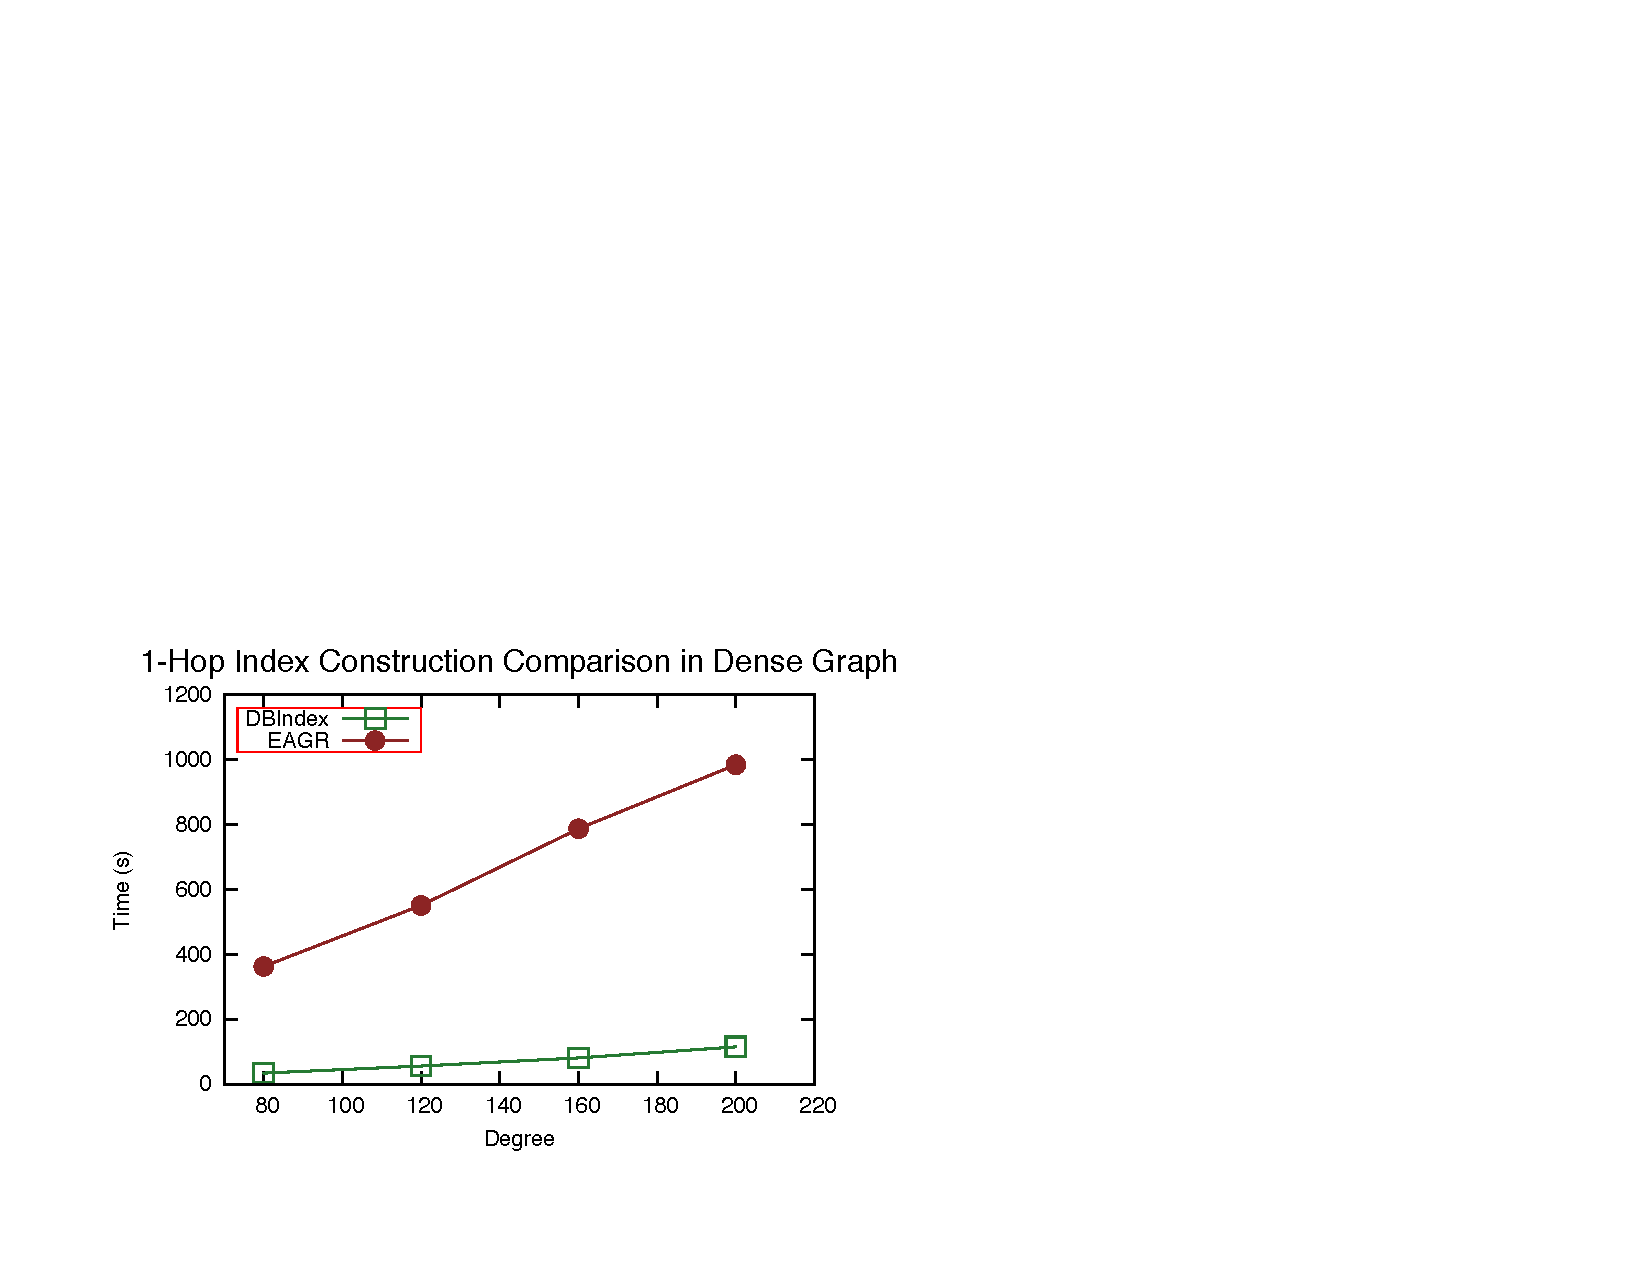
\includegraphics[width=\textwidth]{chapter3/exp/khopeffect/scalability/varyd_index_200k.pdf}
  \caption{Index Construction}
\end{subfigure}
\begin{subfigure}{0.48\linewidth}
  \centering
  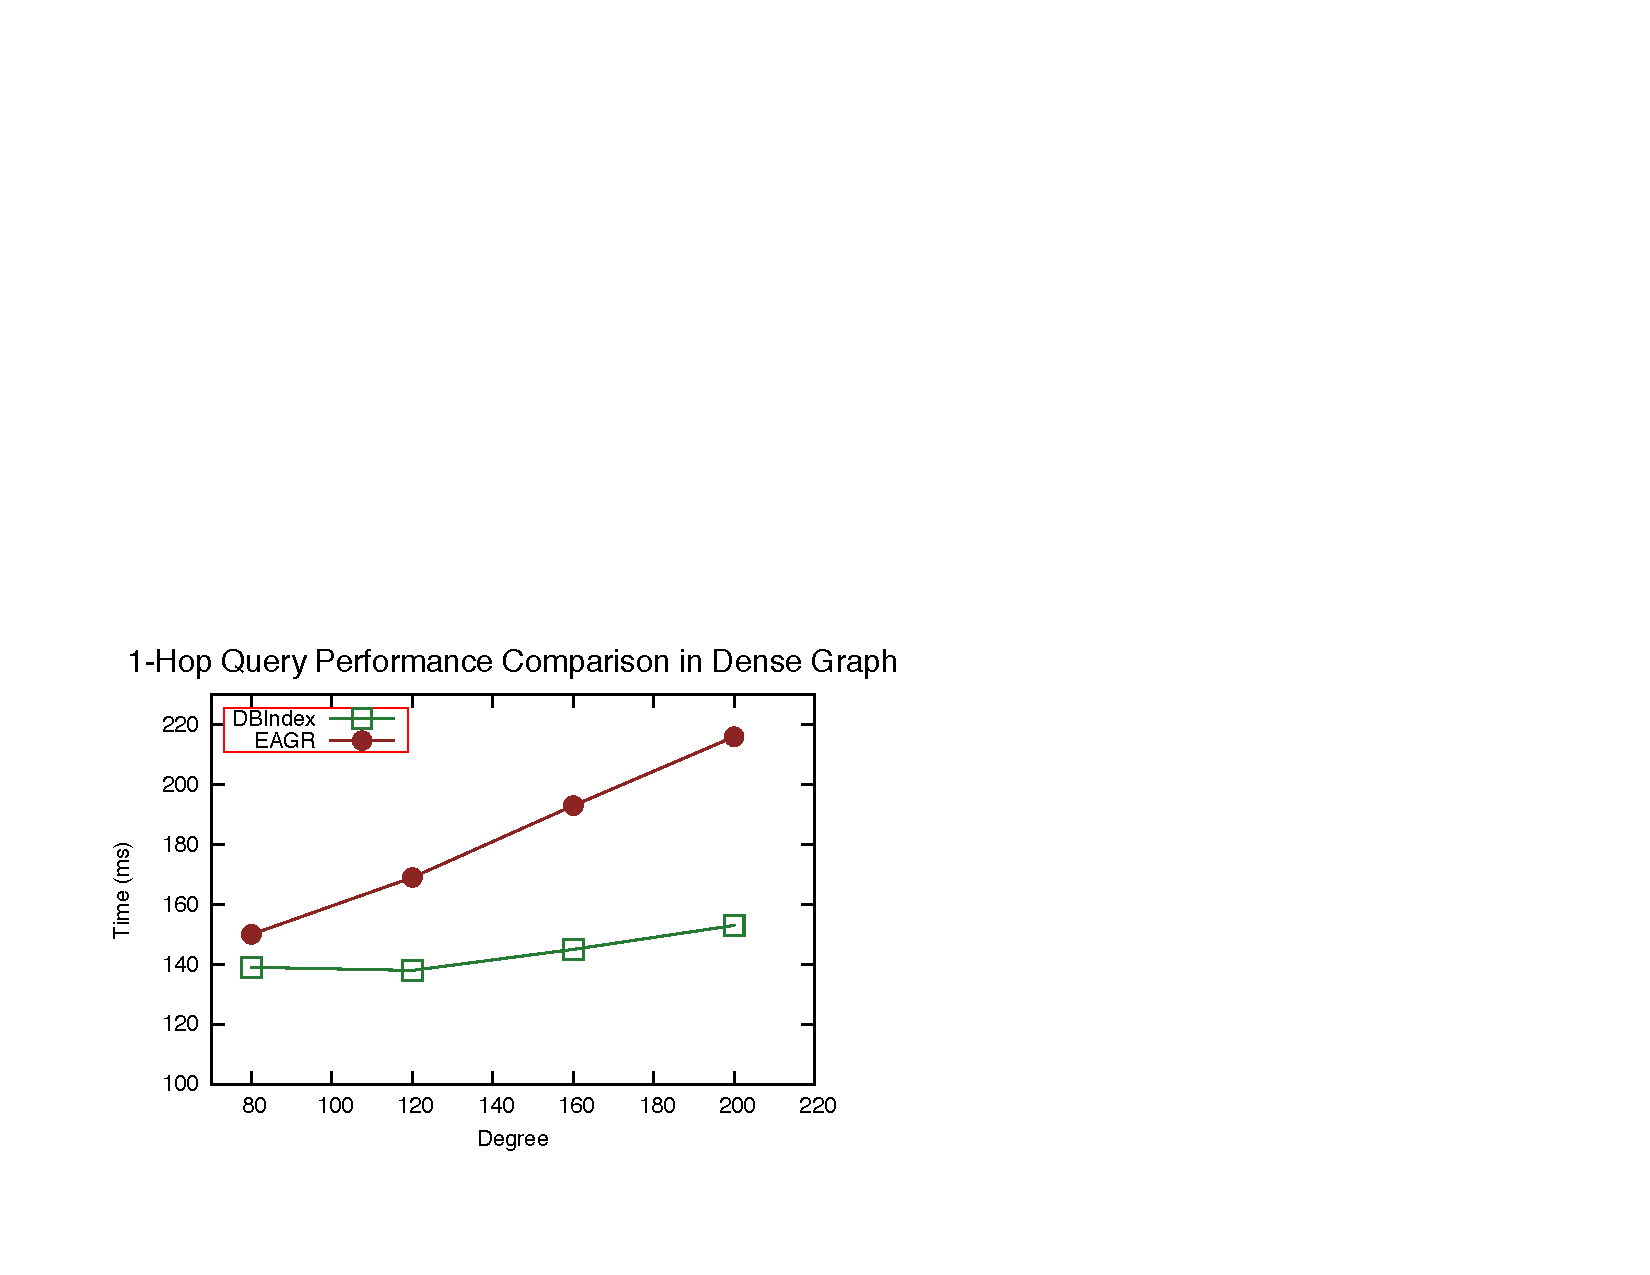
\includegraphics[width=\textwidth]{chapter3/exp/khopeffect/scalability/varyd_query_200k.pdf}
  \caption{Query Performance}
\end{subfigure}
\begin{subfigure}{0.48\linewidth}
  \centering
  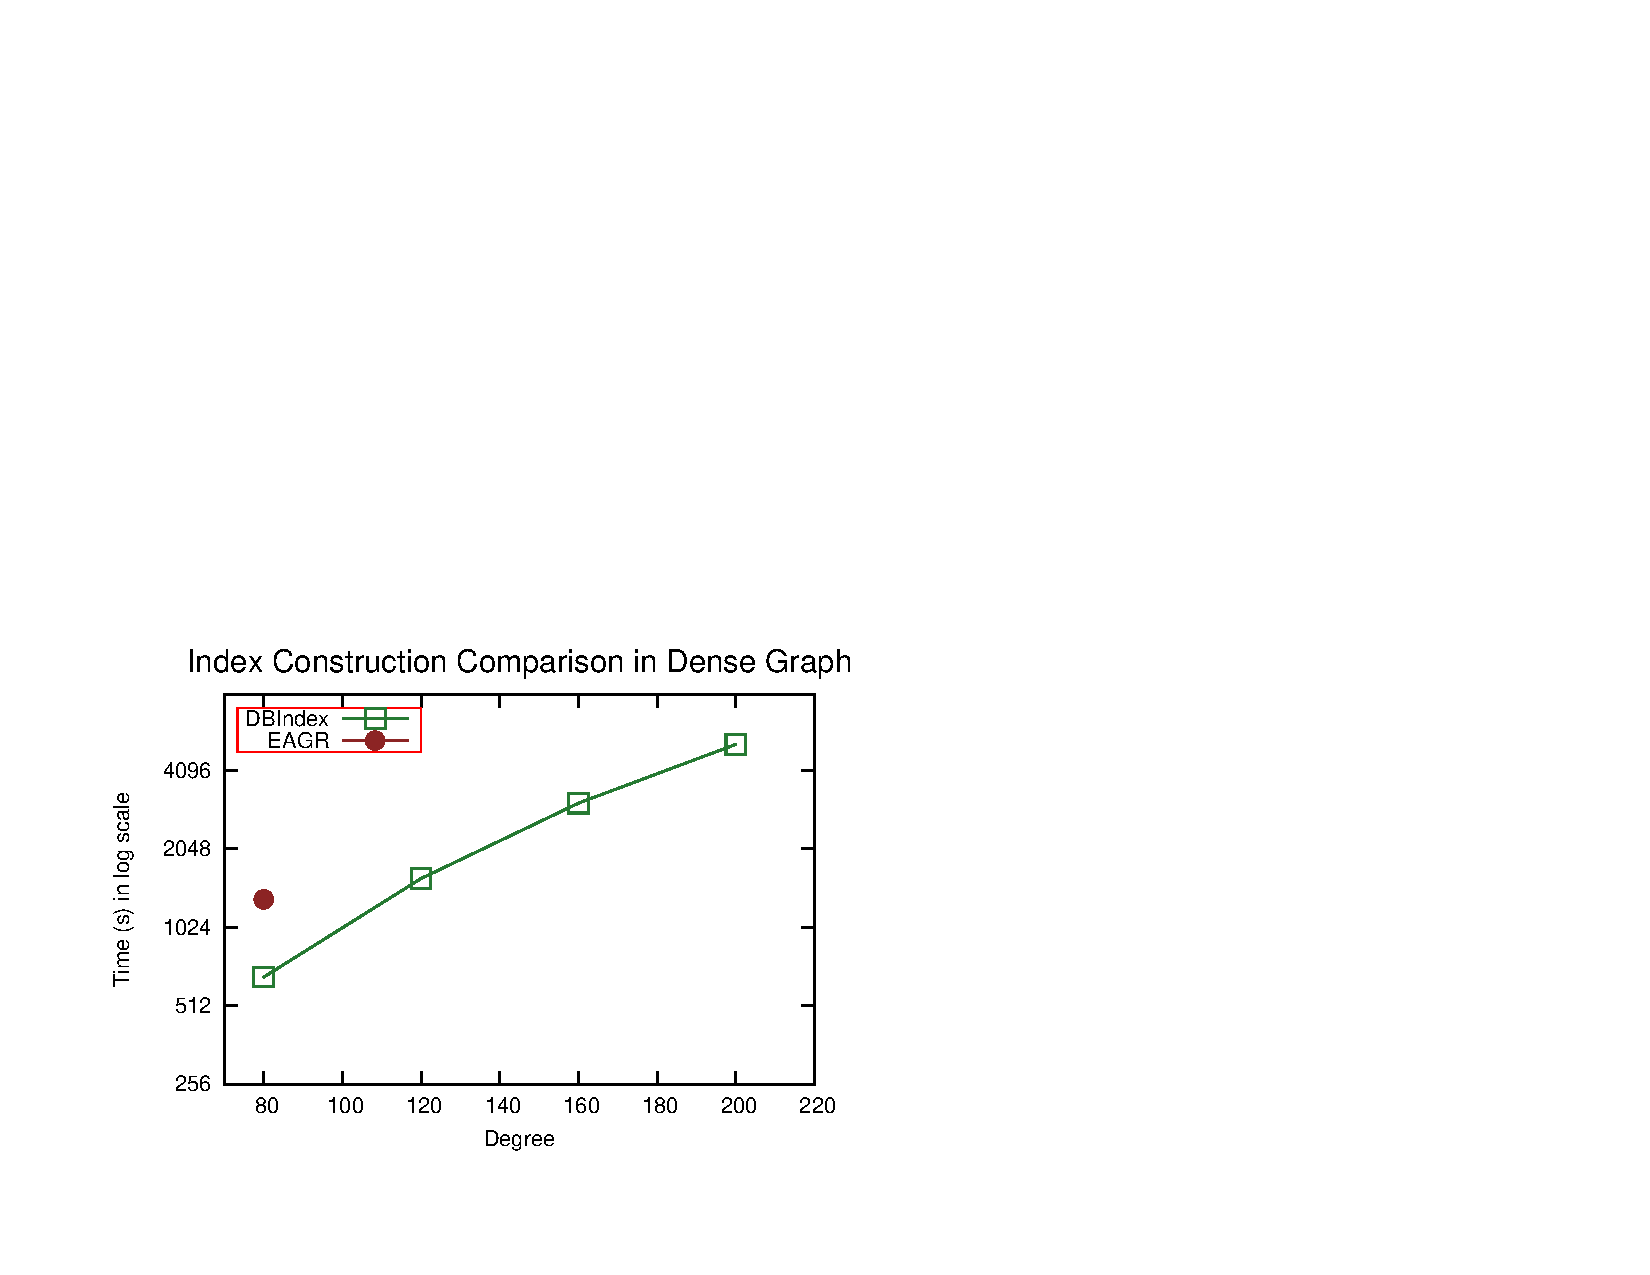
\includegraphics[width=\textwidth]{chapter3/exp/khopeffect/scalability/varyd_index_200k_h2.pdf}
  \caption{Index Construction}
\end{subfigure}
\begin{subfigure}{0.48\linewidth}
  \centering
  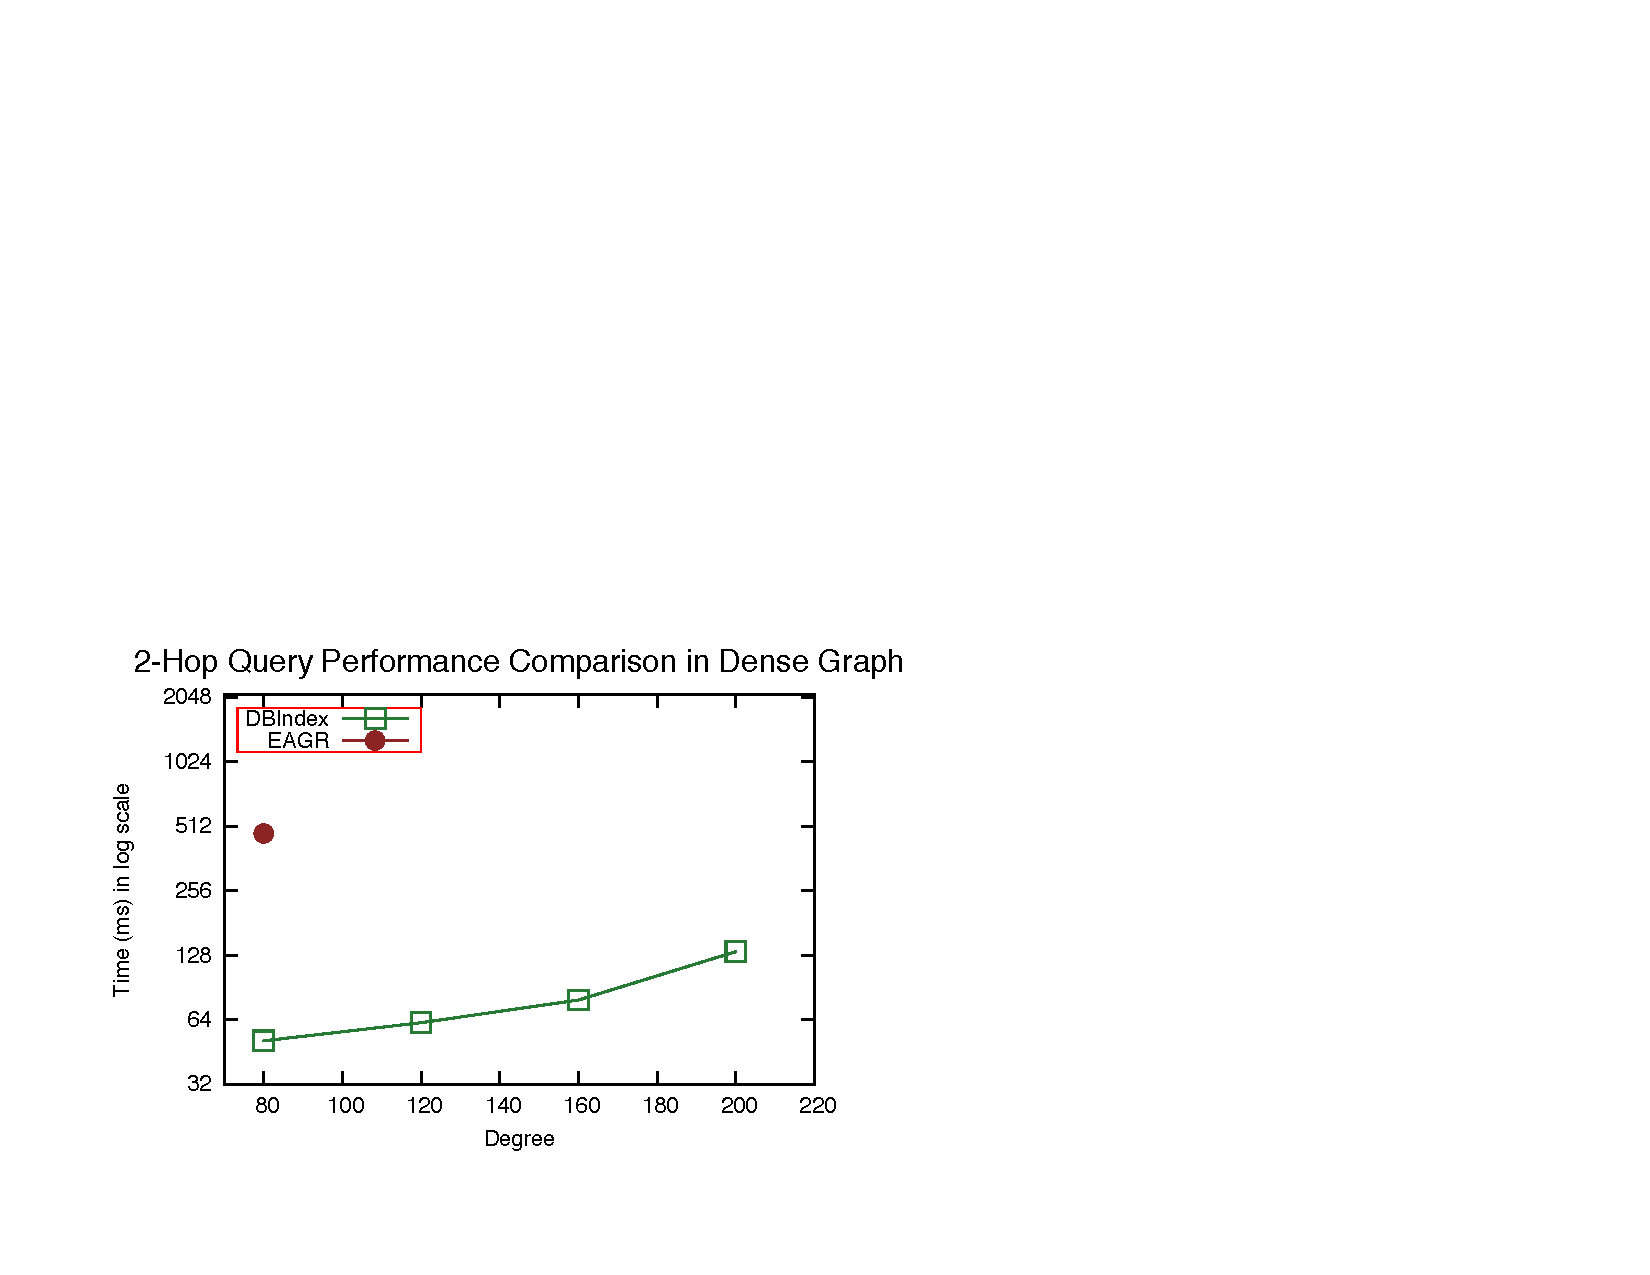
\includegraphics[width=\textwidth]{chapter3/exp/khopeffect/scalability/varyd_query_200k_h2.pdf}
  \caption{Query Performance }
\end{subfigure}
\caption{Impact of Degree over Dense Graphs over 200K Vertices. (a) and (b) are the results for 1-hop query; (c) and (d) are the results for 2-hop query. }
\label{fig:khop_v200k}
\end{figure}

\subsection{Evaluation of I-Index}
In this set of experiments, we evaluate I-Index. 
All the datasets are generated from the DAGGER generator.   

\textbf{Impact of Degree.} First, we evaluate the impact of degree 
changes when we fix the number of vertex as 30k and 60k.  
We compare \emph{DBIndex} with I-Index. 
In the query results, we also implement one non-index algorithm 
which dynamically calculates the window and then performs the aggregation. 
For indexing time, as shown in Figures~\ref{fig:pi_effect} (a) and (c), as the 
index size increases, both the indexing time of 
DBIndex and I-Index increase. However I-Index is more efficient than 
DBIndex, this is due to the special containment optimization used.  We observe that the 
index construction time is almost the same as the one time non-index query time. In other words, 
we can use one query time to create the index which is able to provide much faster query processing for subsequent queries. 
 In terms of query performance, shown in Figs.~\ref{fig:pi_effect} (b) and 
(d), the non-index approach is, on average, 20 times slower than 
the index-based schemes. I-Index outperforms DBIndex by 20\% to 30\%. 
The results clearly show that I-Index outperforms DBIndex for topological 
window in both index construction and query performance. Therefore, in the following experiments, we only present the results for I-Index. 
 
\begin{figure}
\centering
\begin{subfigure}{0.48\linewidth}
  \centering
  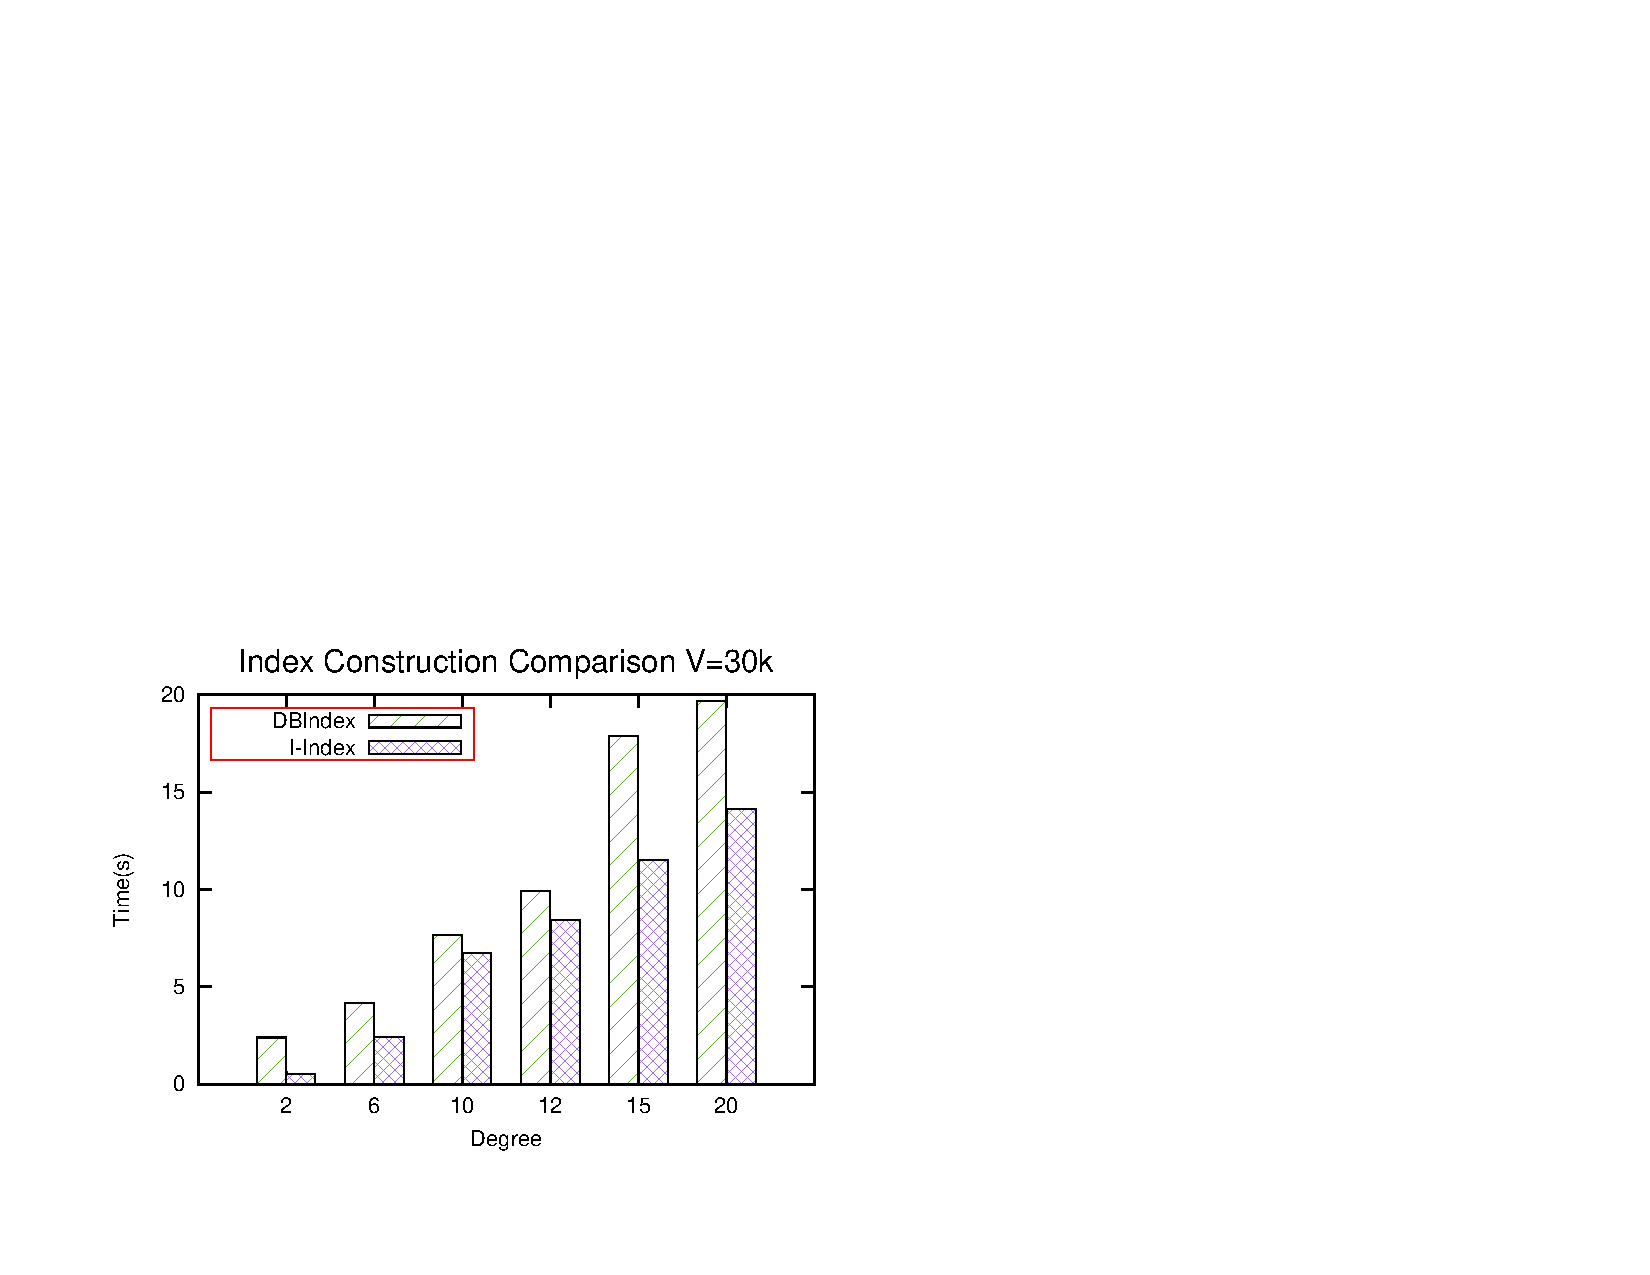
\includegraphics[width=\textwidth]{chapter3/exp/topoeffect/comp/top_index_time_v30k.pdf}
  \caption{Index Construction}
\end{subfigure}
\begin{subfigure}{0.48\linewidth}
  \centering
  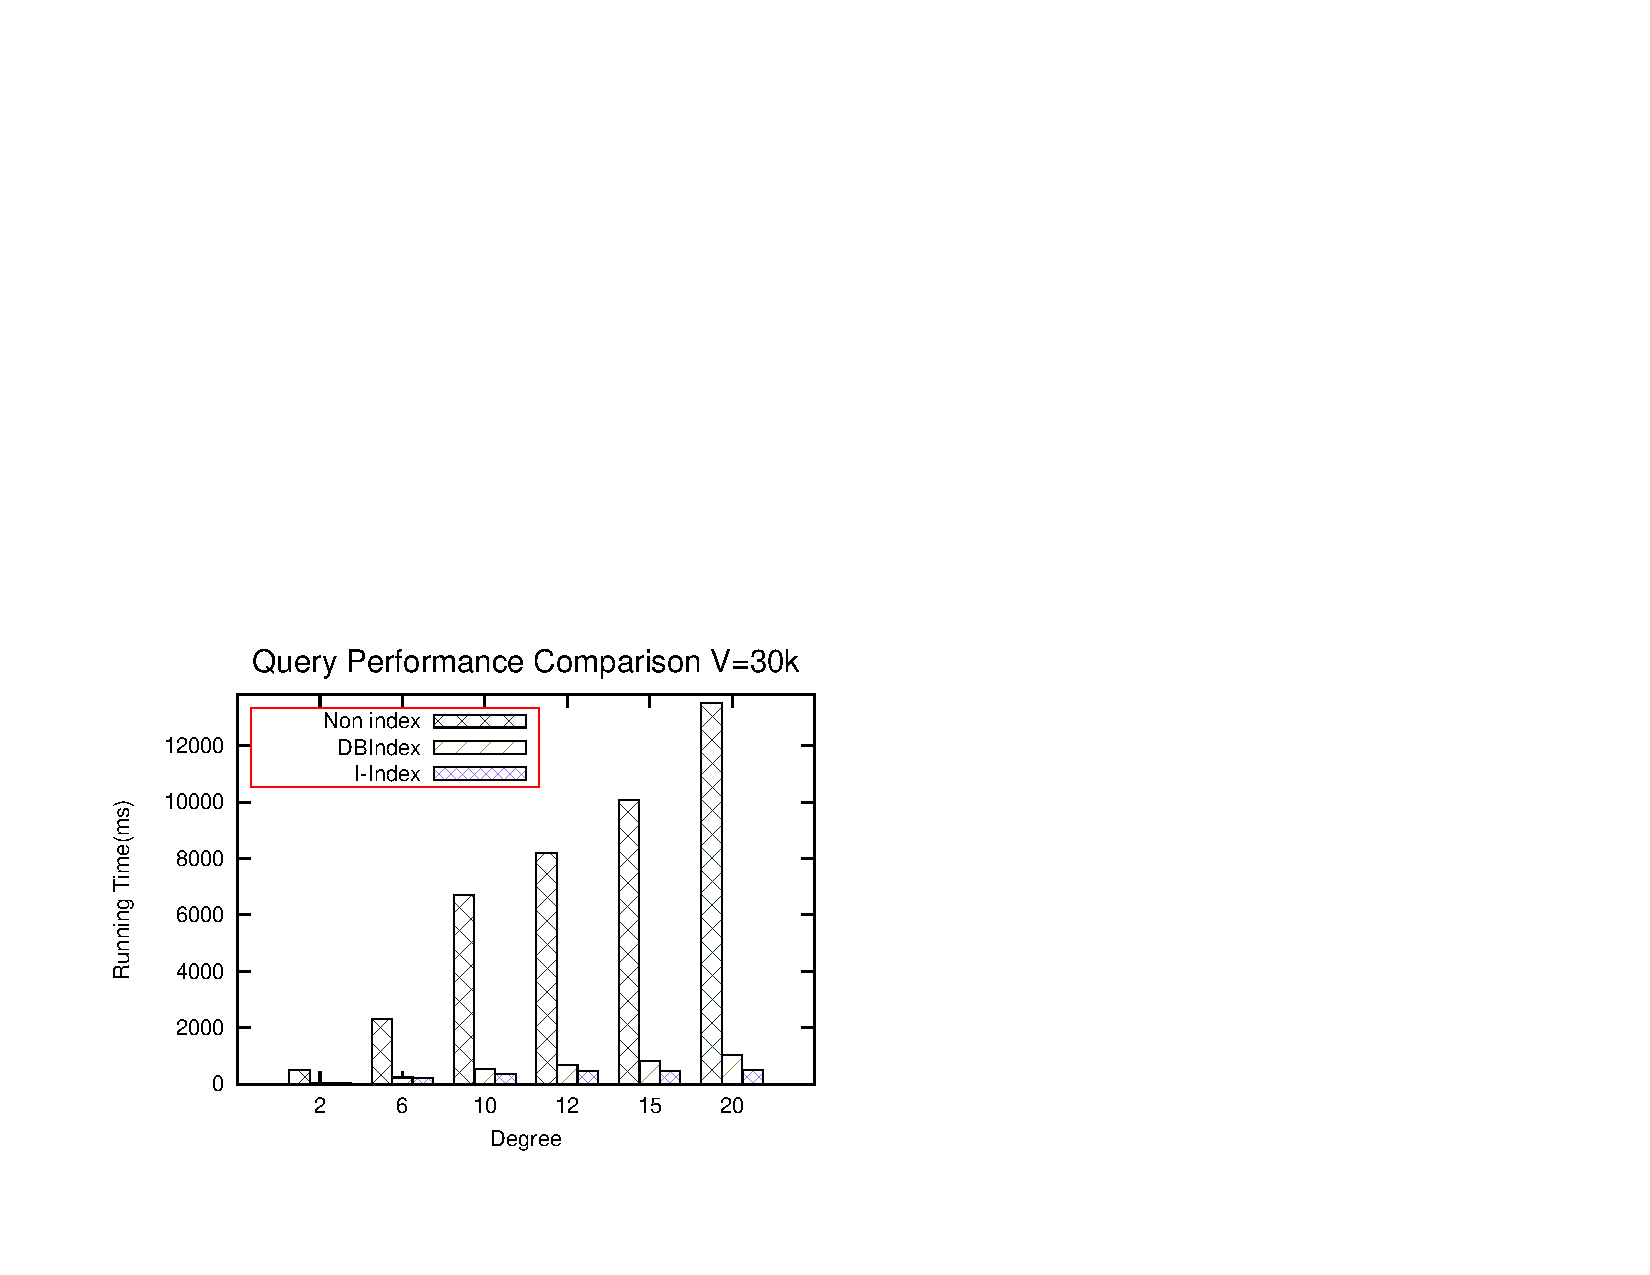
\includegraphics[width=\textwidth]{chapter3/exp/topoeffect/comp/top_query_time_v30k.pdf}
  \caption{Query Performance}
\end{subfigure}
\begin{subfigure}{0.48\linewidth}
  \centering
  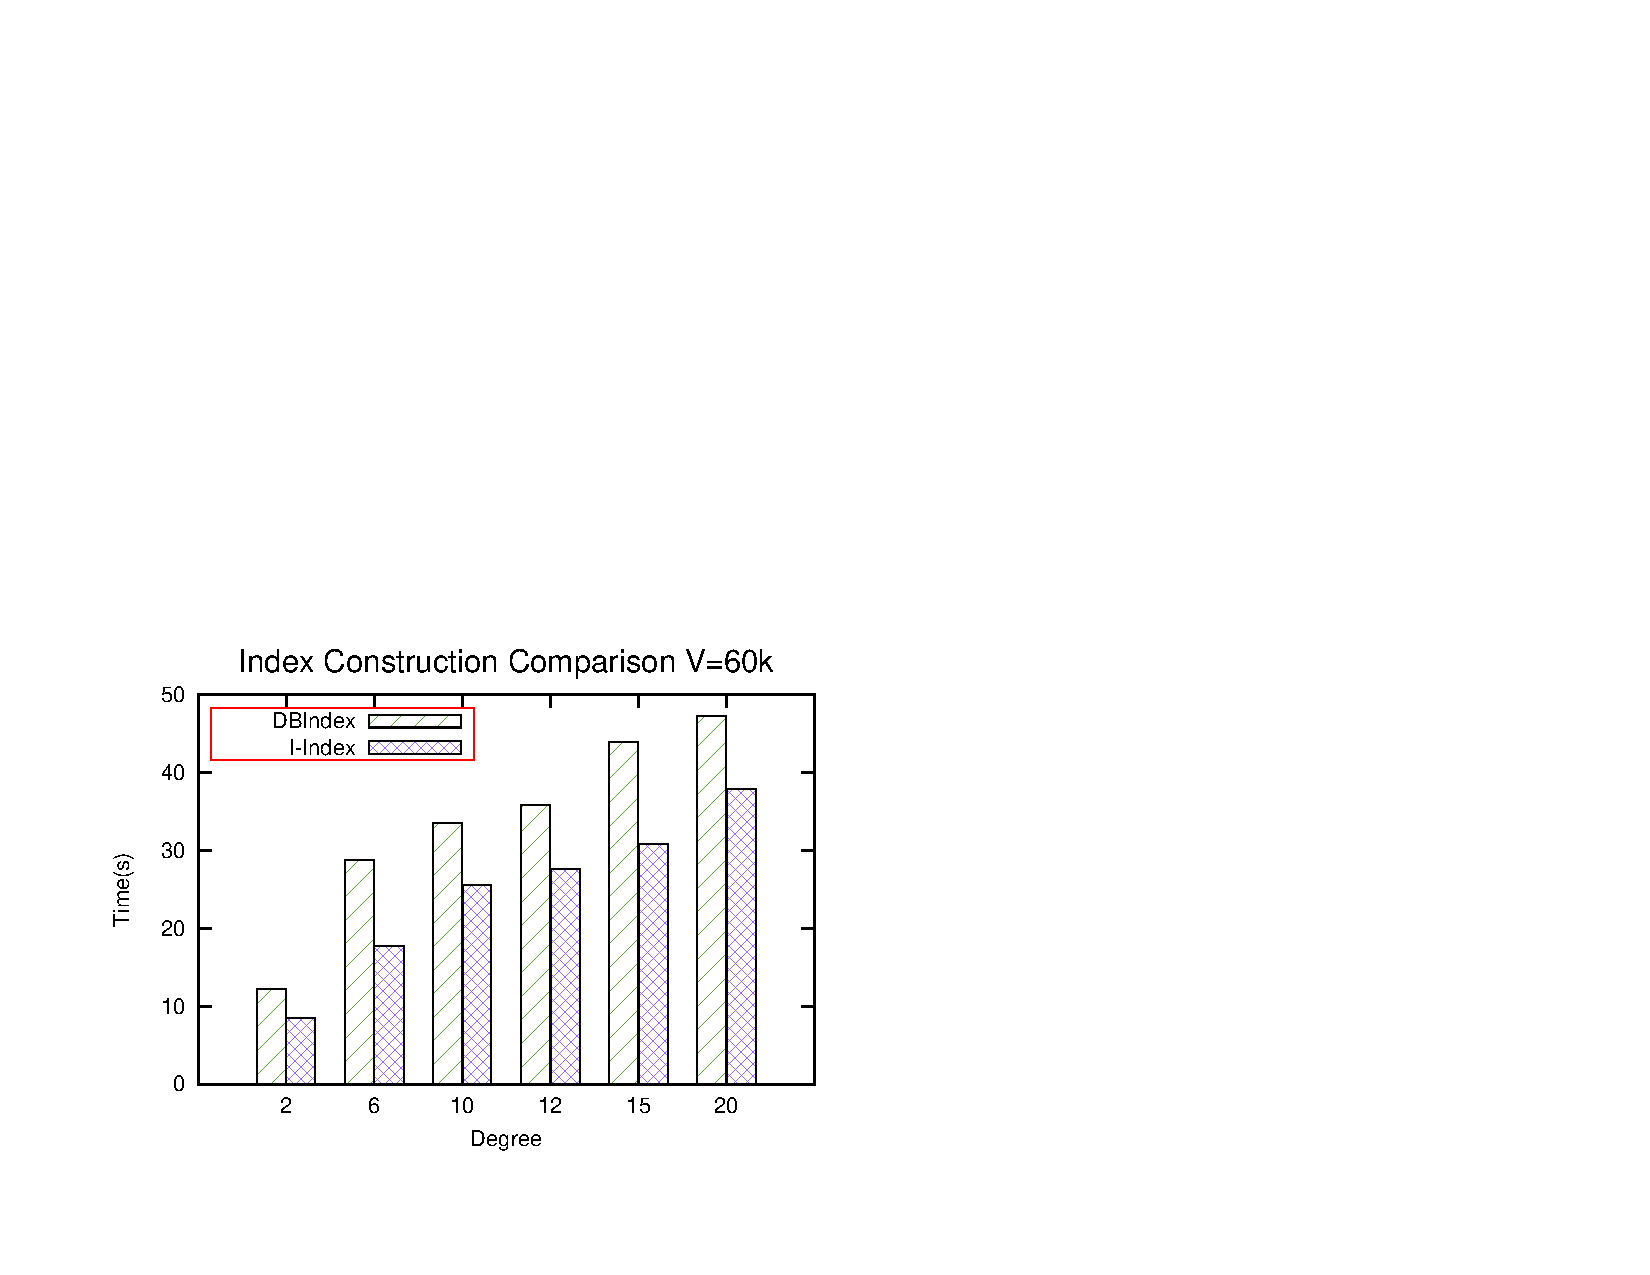
\includegraphics[width=\textwidth]{chapter3/exp/topoeffect/comp/top_index_time_v60k.pdf}
  \caption{Index Construction}
\end{subfigure}
\begin{subfigure}{0.48\linewidth}
  \centering
  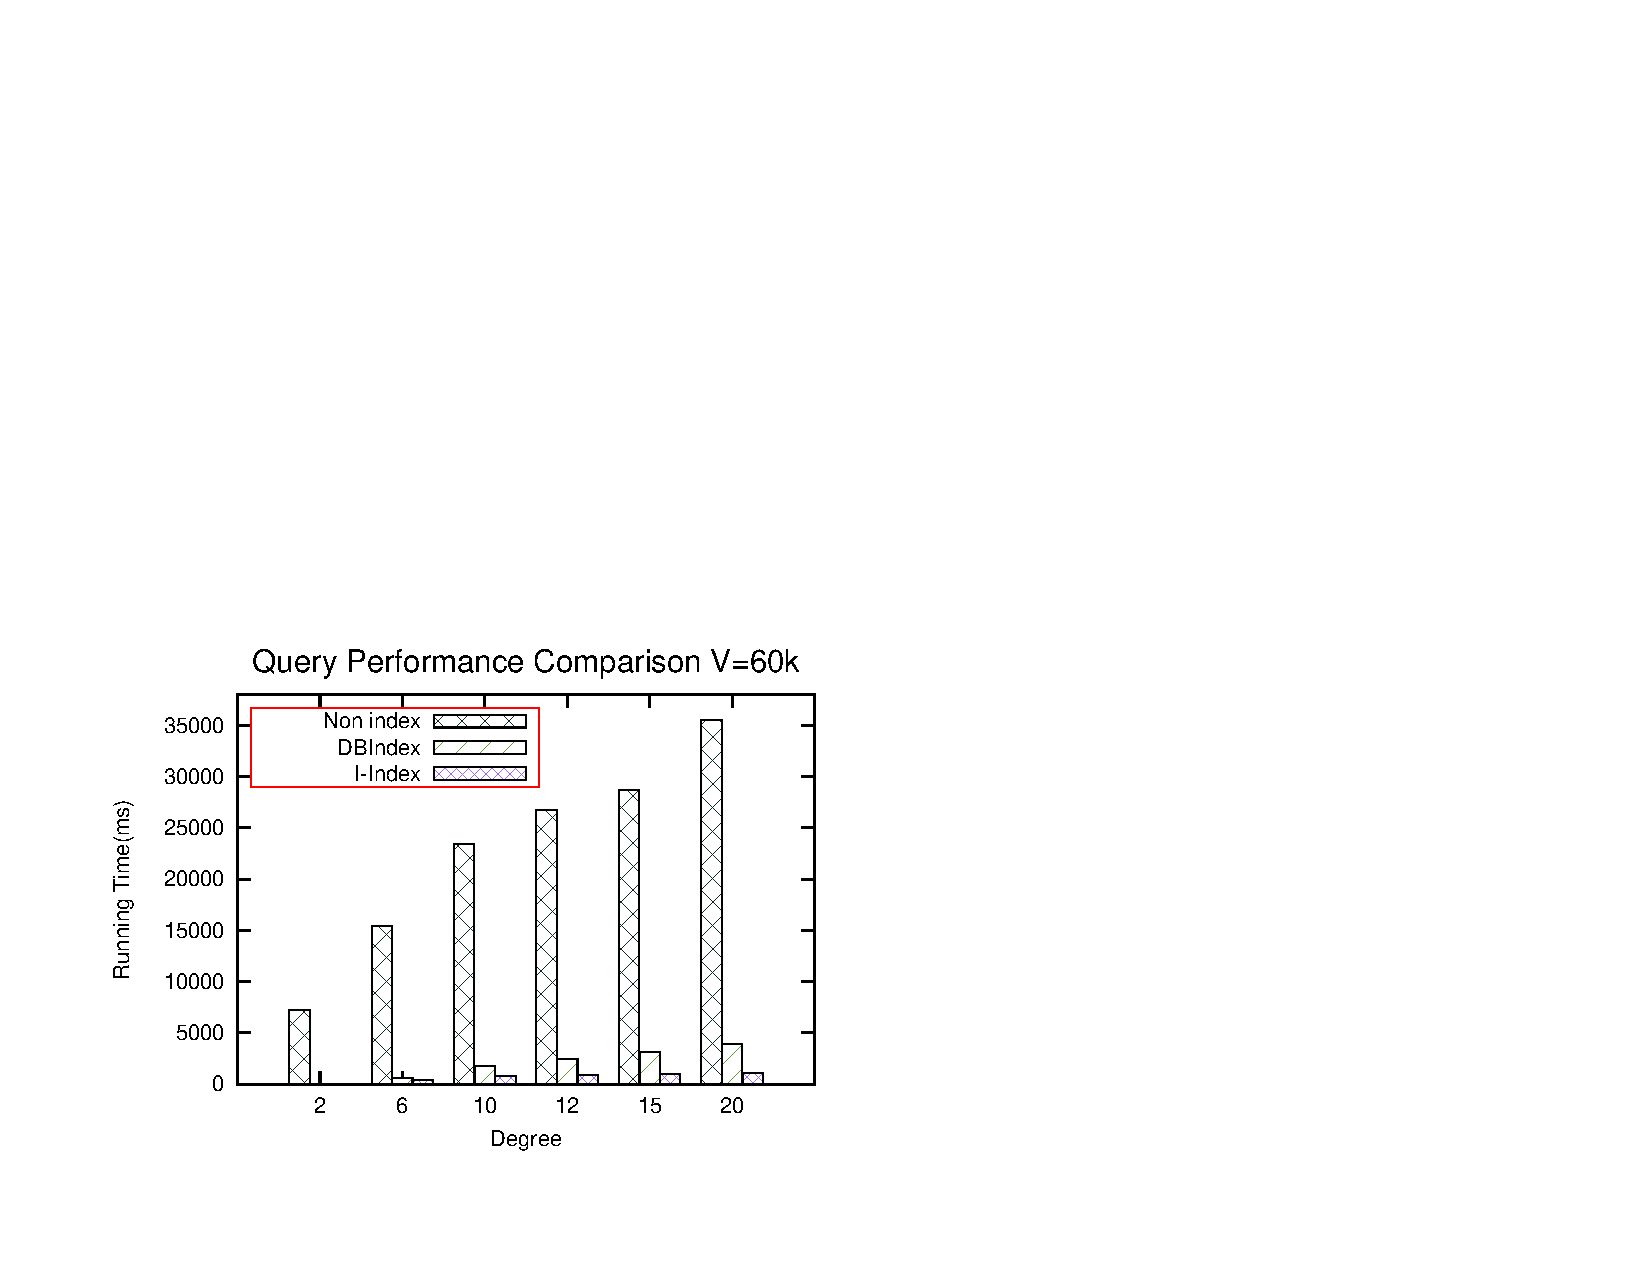
\includegraphics[width=\textwidth]{chapter3/exp/topoeffect/comp/top_query_time_v60k.pdf}
  \caption{Query Performance}
\end{subfigure}
\caption{Impact of Degree. (a) and (b) are the results for 30K vertices; (c) and (d) are the results for 60K vertices.}
\label{fig:pi_effect}
\end{figure}


\textbf{Impact of Number of Vertices.} Next, we study how the performance of I-Index 
 is affected when we fix the degree and vary the number of vertices from 50k to 350K. 
Figs.~\ref{fig:pi_effect2} (a) and (c) show the index construction time when we fix the degree to 
10 and 20 respectively. From the results, we see that the construction time increases while the number of vertex increases and the construction time of a high degree graph is longer than that for low degree graphs. Figs.~\ref{fig:pi_effect2} (b) and (d) show the query time when we fix the degree to 10 and 20 respectively. 
As shown, the degree affects the query processing time - when the degree increases, the query time increases as well. We also observe that the query time is increasing linearly when the number of vertices increases. This shows the I-Index has good scalability.  

\textbf{Index Size.} Fig.~\ref{fig:top-index-size} presents
the index size ratio (i.e. size of index divided by the size of original graph) under different degrees from 3 to 20. 
There are four different sizes of data used with 100k, 150k, 200k and 300k vertices.  
For every vertex setting, the index size maintains the same trend in various degrees. The index size is linear to the input graph size. 
As a graph gets denser, the difference field of the I-Index
effectively shrinks. Thus, the index size in turn becomes smaller, which explains the bends in the figure.

\begin{figure}
\centering
\begin{subfigure}{0.48\linewidth}
  \centering
  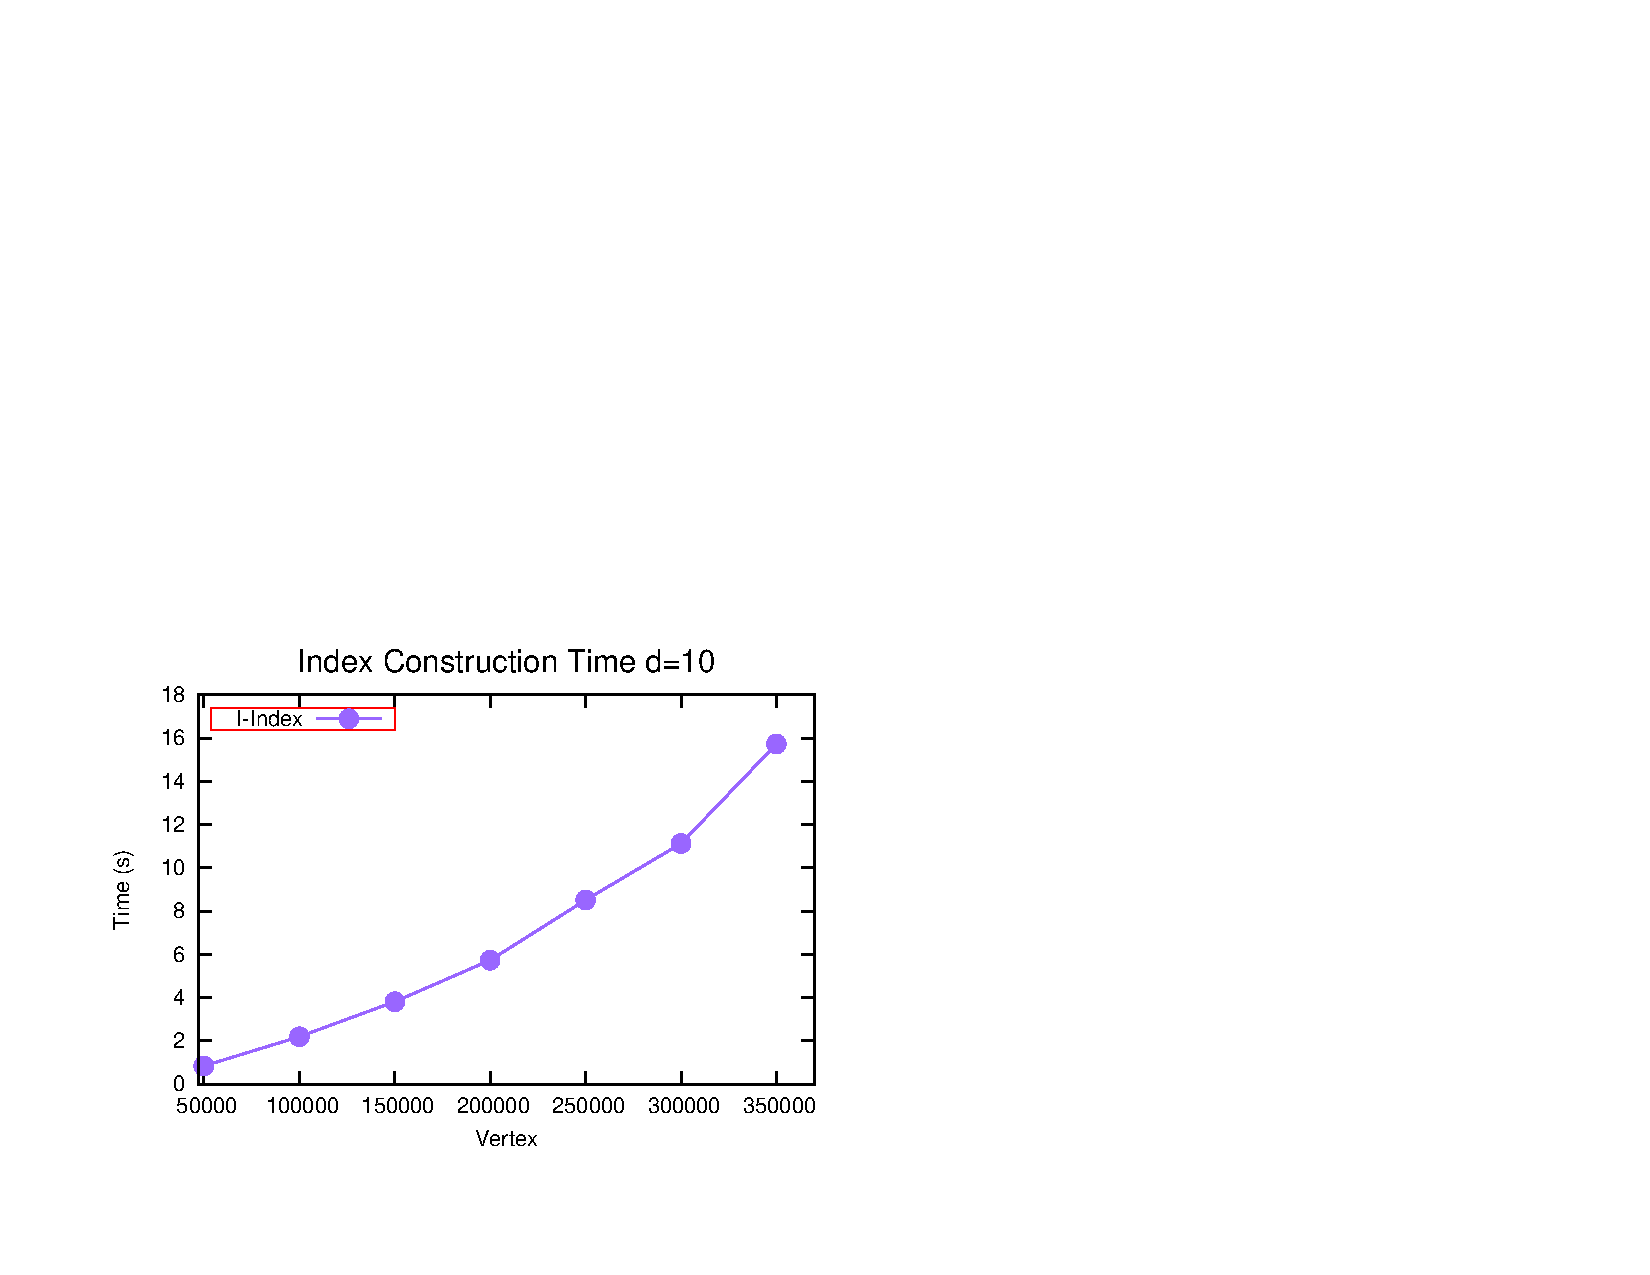
\includegraphics[width=\textwidth]{chapter3/exp/topoeffect/comp/top_scale_index_d10.pdf}
  \caption{Index Construction }
\end{subfigure}
\begin{subfigure}{0.48\linewidth}
  \centering
  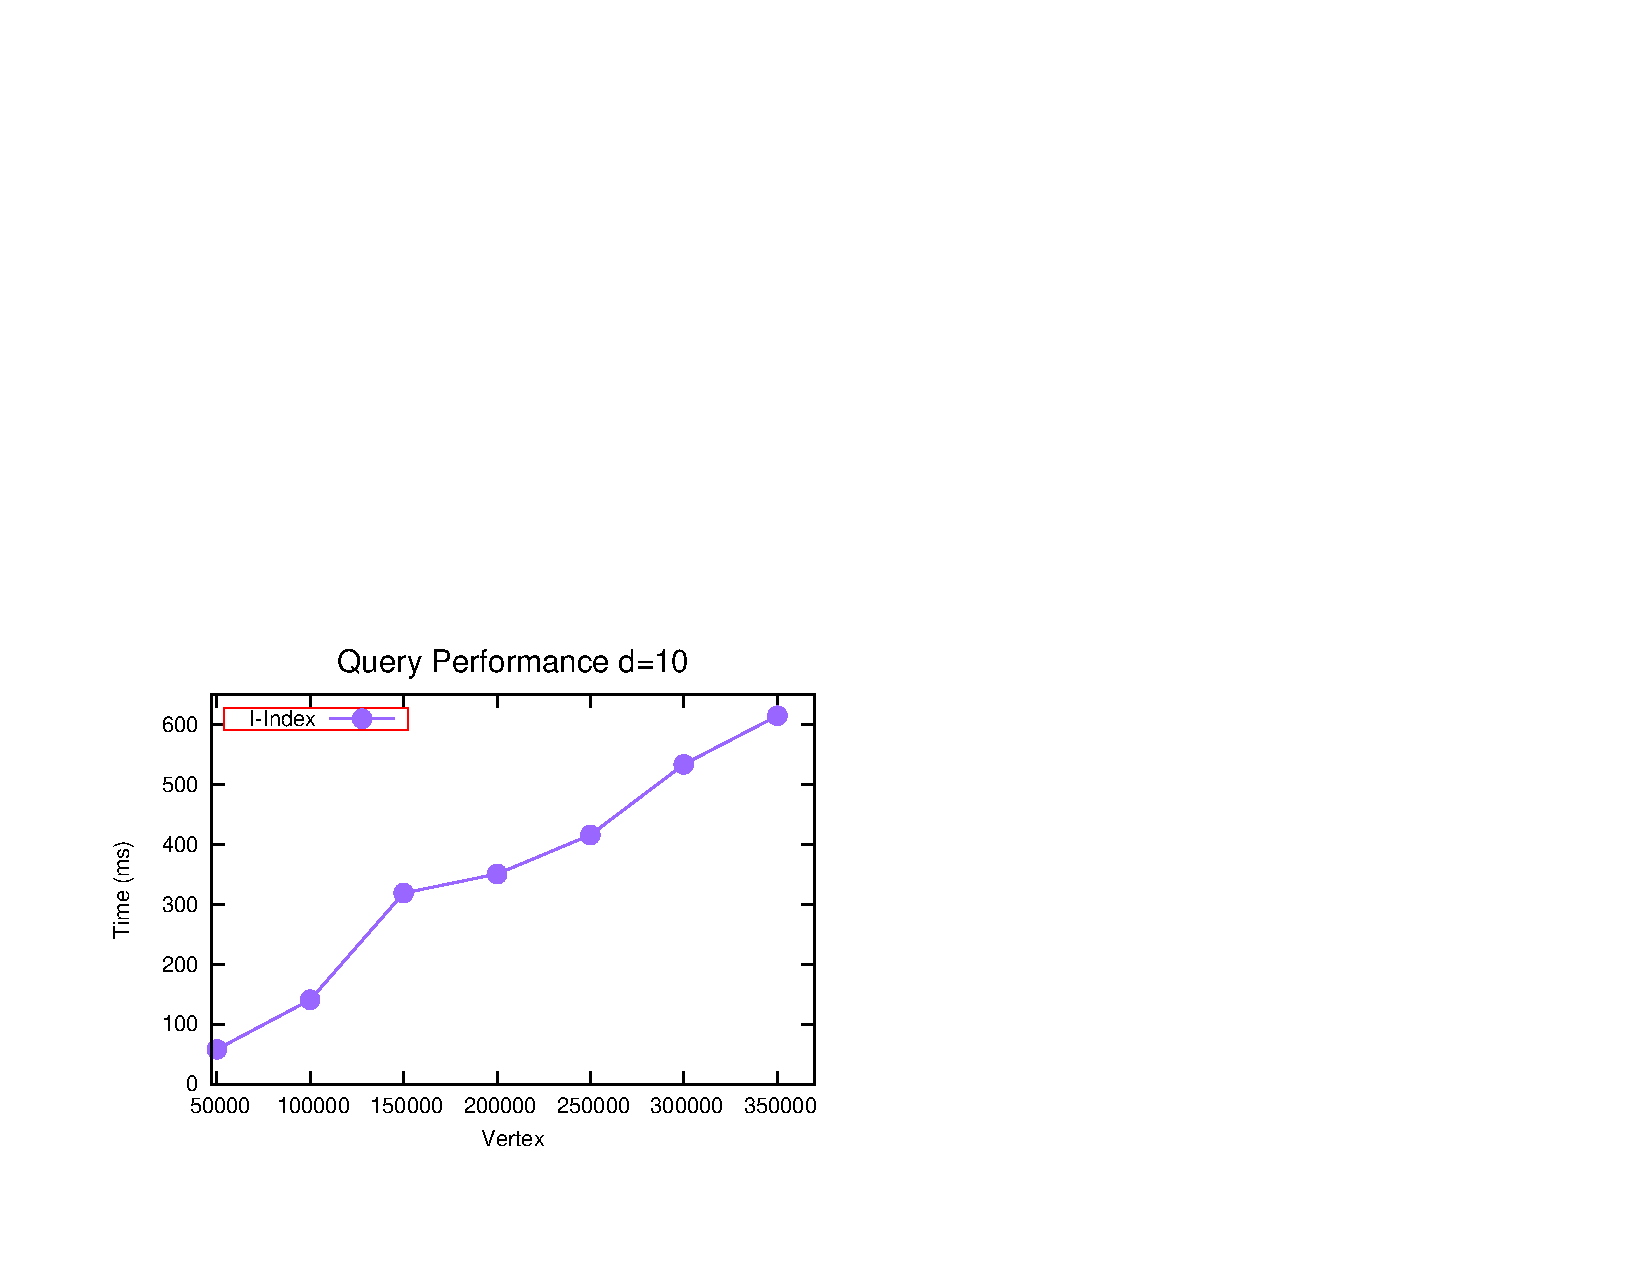
\includegraphics[width=\textwidth]{chapter3/exp/topoeffect/comp/top_scale_query_d10.pdf}
  \caption{Query Performance}
\end{subfigure}
\begin{subfigure}{0.48\linewidth}
  \centering
  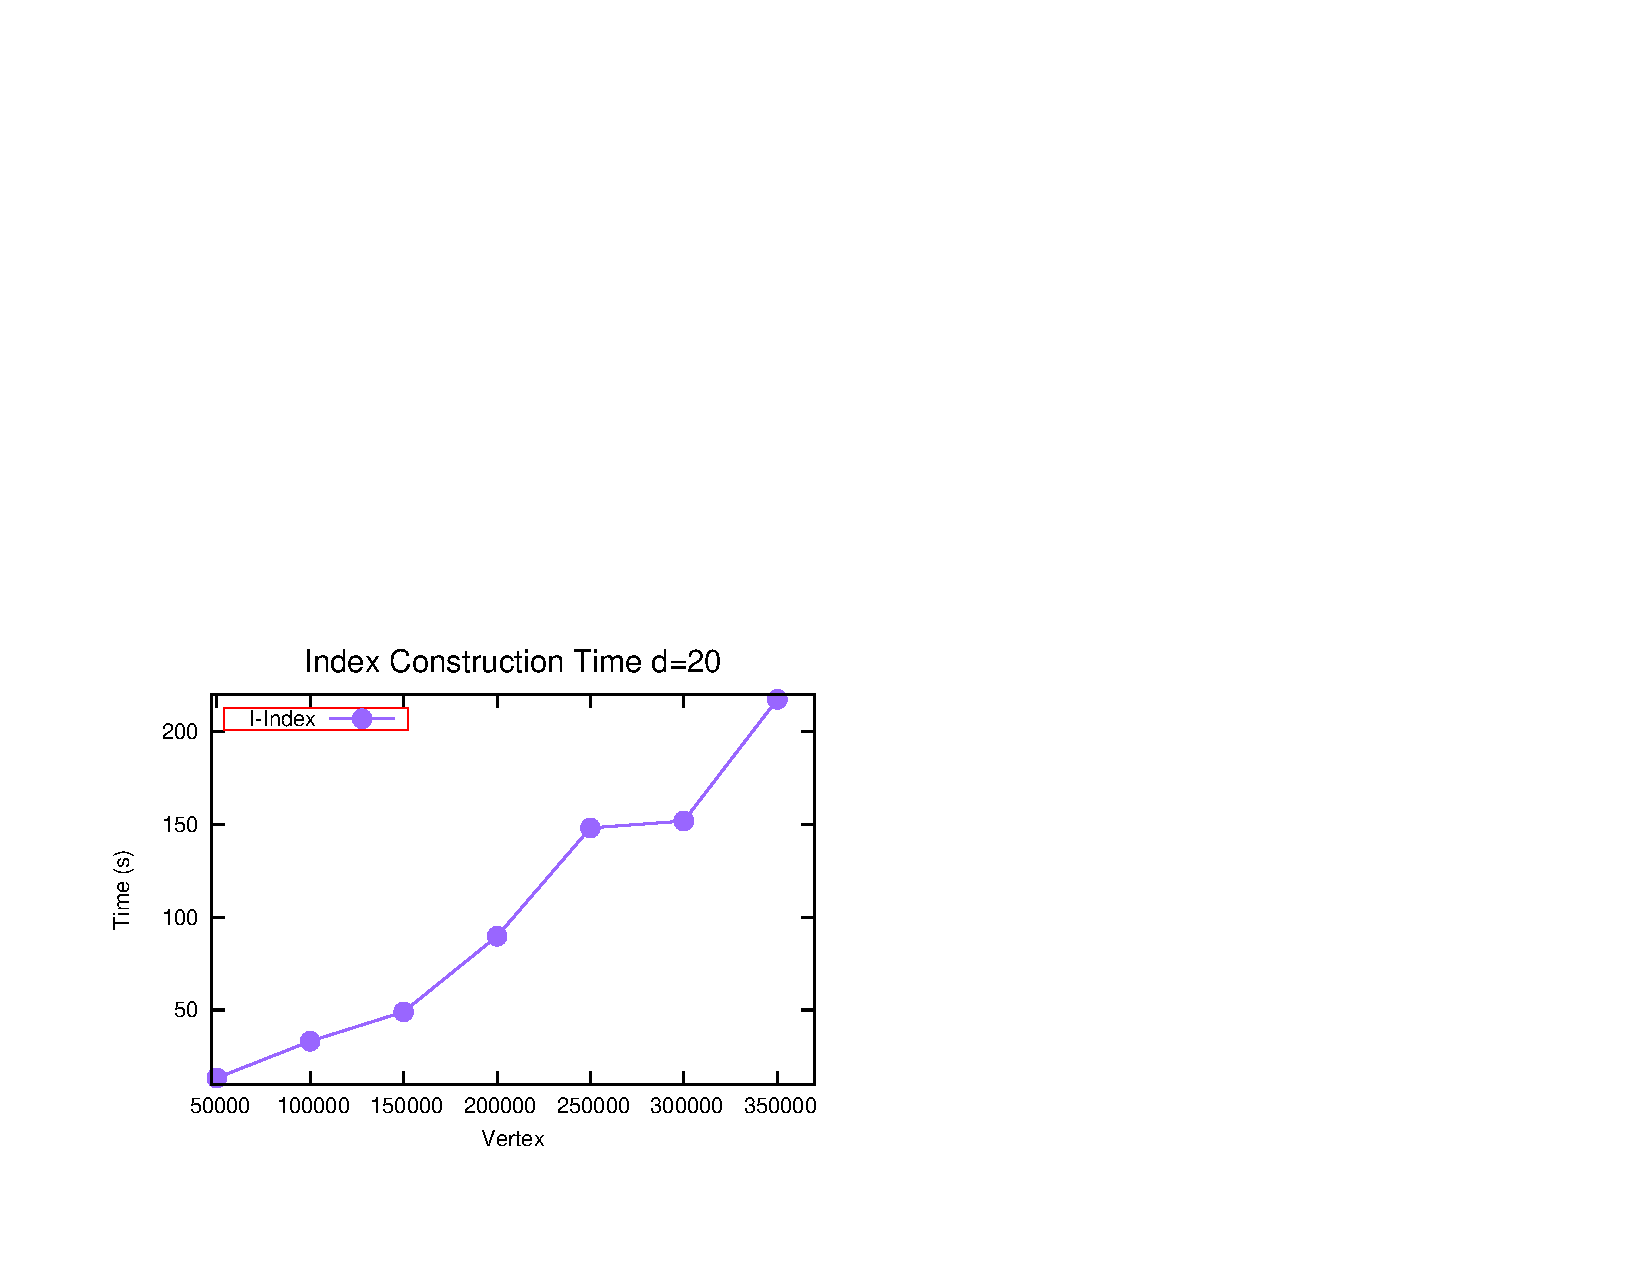
\includegraphics[width=\textwidth]{chapter3/exp/topoeffect/comp/top_scale_index_d20.pdf}
  \caption{Index Construction}
\end{subfigure}
\begin{subfigure}{0.48\linewidth}
  \centering
  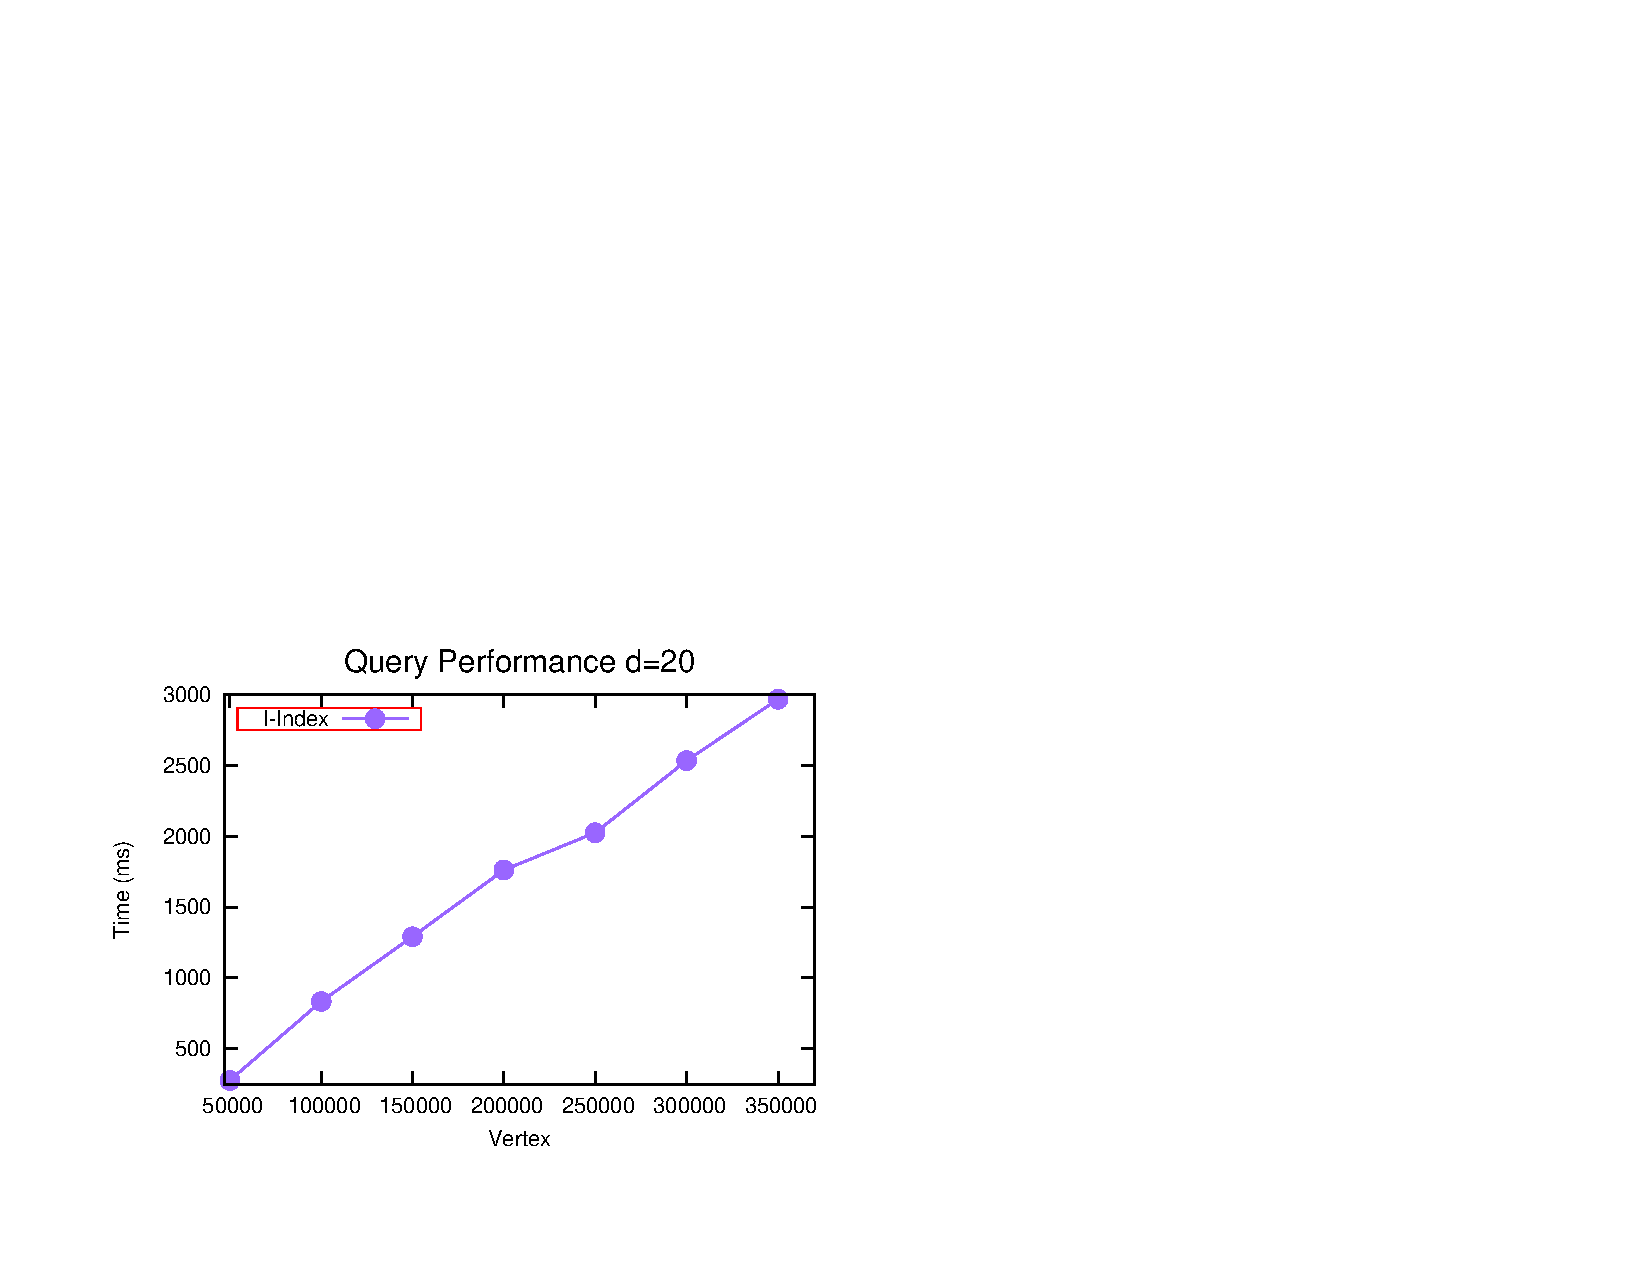
\includegraphics[width=\textwidth]{chapter3/exp/topoeffect/comp/top_scale_query_d20.pdf}
  \caption{Query Performance}
\end{subfigure}
\caption{Impact of the number of vertices with a fixed degree. (a) and (b) 
are the results for the graphs with degree 10; (c) and (d) 
are the graphs with degree 20. }
\label{fig:pi_effect2}
\end{figure}

\begin{figure}[h]
\centering
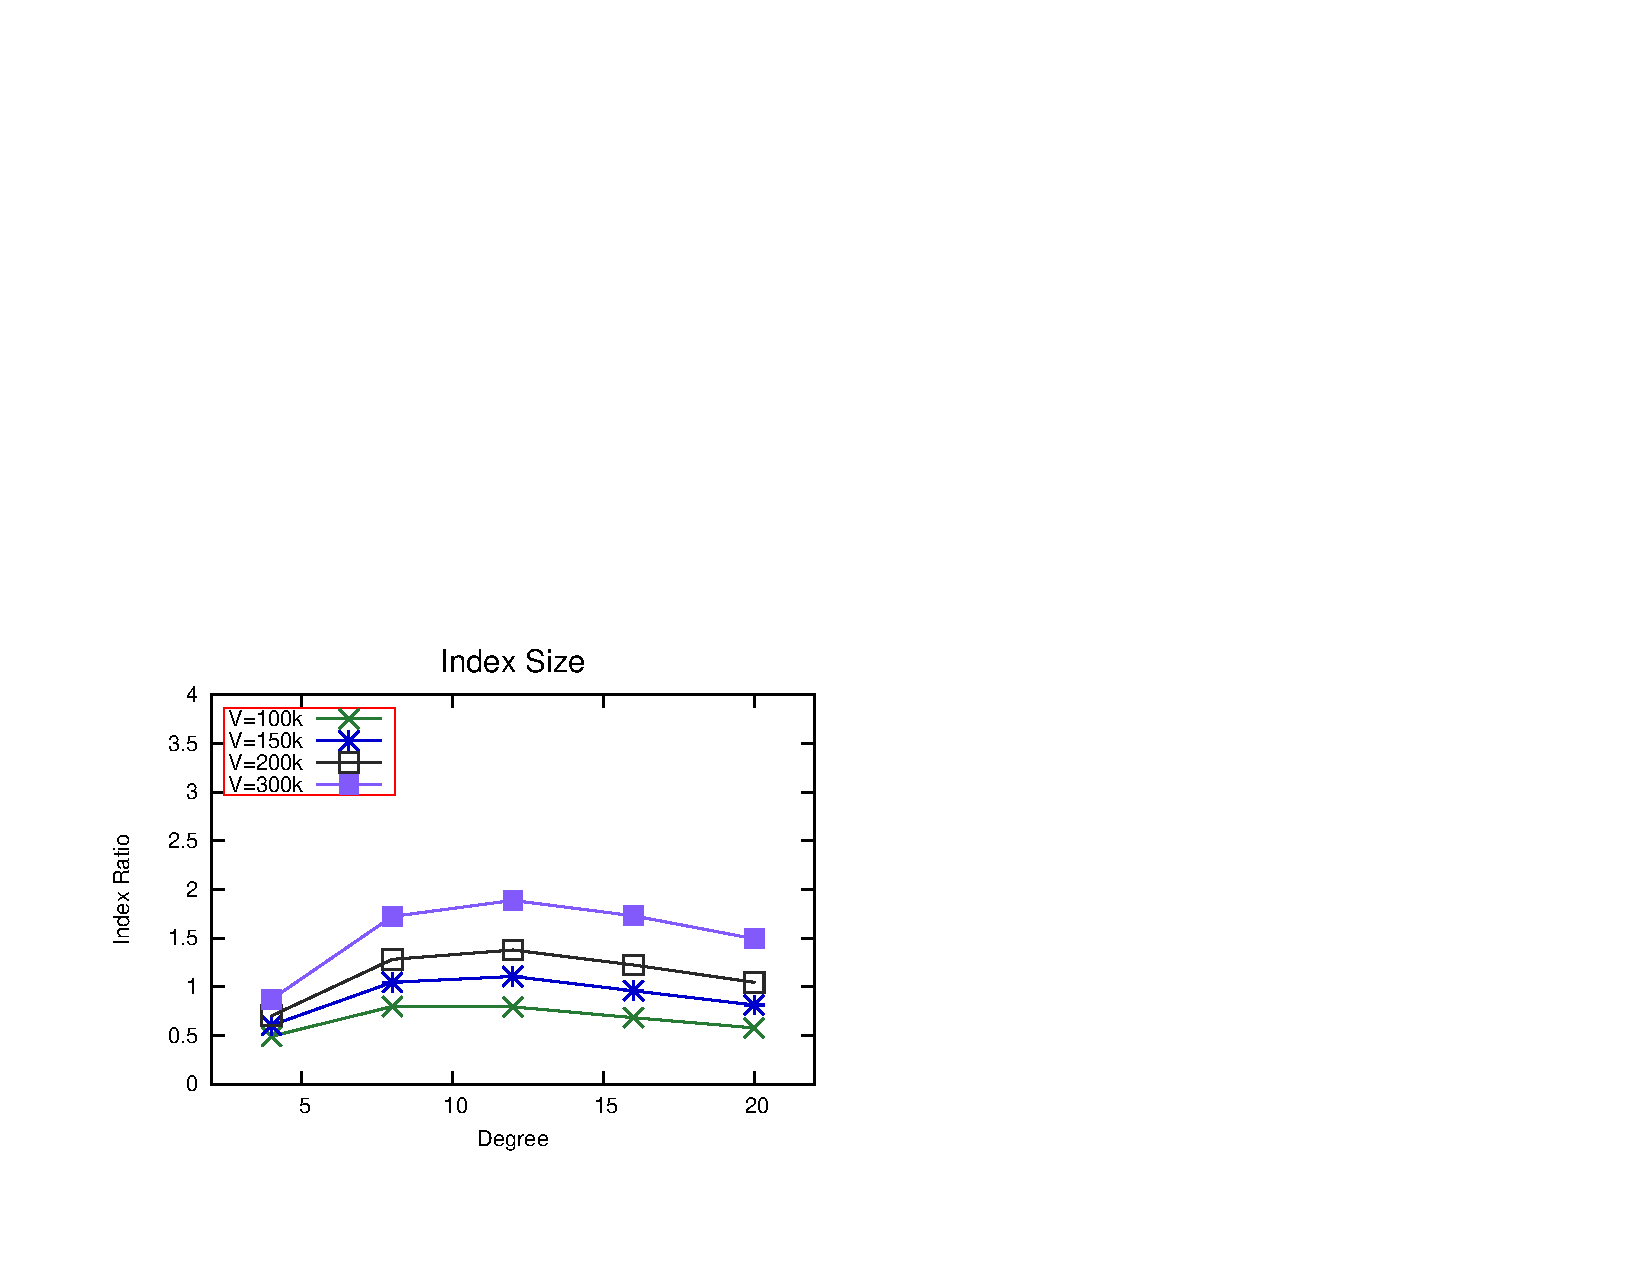
\includegraphics[width=0.5\textwidth]{chapter3/exp/topoeffect/comp/top_scale_index_size.pdf}
\caption{Index Ratio of Inheritance-Index}
\label{fig:top-index-size}
\end{figure}


